\documentclass[12pt]{article}
%\renewcommand{\baselinestretch}{1.15}
\usepackage{natbib,amsmath,amsthm,booktabs,subfigure,anysize,hyperref,graphicx,float,bbm,epstopdf}
\usepackage[margin=1in]{geometry}
\bibliographystyle{aea}
%\bibliographystyle{apalike}
%\bibliographystyle{aernobold}
%\bibliographystyle{economet}
%\marginsize{2cm}{2cm}{2cm}{2cm}

\usepackage{threeparttable}
\usepackage{array} % for adding extra space between table columns
\usepackage{booktabs} % for adding extra space between table columns
\usepackage{multirow}
\usepackage{xcolor}
\usepackage{bm}
\definecolor{dark-red}{rgb}{0.4,0.15,0.15}
\definecolor{dark-blue}{rgb}{0.15,0.15,0.4}
\definecolor{medium-blue}{rgb}{0,0,0.5}
\definecolor{ChadBlue}{rgb}{.1,.1,.5}
% Chad's colors:
% See http://web.njit.edu/~kevin/rgb.txt.html for possibilities
\definecolor{ChadDarkBlue}{rgb}{.1,0,.1}
\definecolor{ChadBlue}{rgb}{.1,.1,.5}
\definecolor{ChadRoyal}{rgb}{.2,.2,.8}
%\definecolor{ChadGreen}{rgb}{0,.35,.1}
%\definecolor{ChadGreen}{rgb}{0,.5,.25}  % Too bright
%\definecolor{ChadGreen}{rgb}{0,.4,.2}    % Still too bright
\definecolor{ChadGreen}{rgb}{0,.4,0}    % Dark Green
%\definecolor{ChadRed}{rgb}{.8,.1,.2}    % Too bright
\definecolor{ChadRed}{rgb}{.5,0,.5}  % purple
\hypersetup{
    colorlinks, linkcolor=ChadRed,
    citecolor=ChadBlue, urlcolor=ChadBlue
}
\newcommand\posscite[1]{\citeauthor{#1}'s (\citeyear{#1})}
\setlength{\parskip}{0.12cm}
\newtheorem{proposition}{\color{ChadGreen} Proposition}
\newtheorem{finding}{\color{ChadGreen} Finding}
\newtheorem{SF}{\color{ChadGreen} Stylized fact}
\newtheorem{hyp}{Hypothesis}
\newtheorem{fact}{Fact}
\newtheorem{prop}{Proposition}
\usepackage{caption}
%\usepackage[font=small,labelfont={color=ChadBlue,bf}]{caption}
\usepackage[font=small,labelfont=bf]{caption}
%\usepackage{subcaption}
%\usepackage{subfloat}
\usepackage{amssymb}
\usepackage{amsfonts}
\usepackage{amsmath}
\usepackage{accents}
\usepackage{color,soul}
\usepackage{smartdiagram}
\usepackage[figuresright]{rotating} % Rotating table
\usepackage{lscape} % Rotating table
\usepackage{diagbox}
\usepackage{multicol}
\usepackage{tikz}
\usepackage{comment}
\usepackage{float}

\newcommand{\ubar}[1]{\underaccent{\bar}{#1}}
\usepackage{setspace}  %using this package conflicts with footnote hyperlink jump. Using this package makes the footnote links inactive.
\usepackage[all]{hypcap}        % needed to help hyperlinks direct correctly;
%\renewcommand{\sfdefault}{ptm}

\newtheorem{theorem}{Theorem}
\newtheorem{cor}[theorem]{Corollary}
\renewcommand{\proof}{\noindent \textbf{Proof.\ }}
\newtheorem{conjecture}{Conjecture}
\newtheorem{example}{Example}
\newtheorem{defn}{Definition}
\renewcommand{\qed}{\hfill\rule{2.1mm}{2.1mm}}
%\newtheorem{proposition}{\color{ChadGreen} Proposition}
%\newtheorem{finding}{\color{ChadGreen} Finding}
%\newtheorem{SF}{\color{ChadGreen} Stylized fact}
% Fix title, sections, etc.
\newcommand\fnote[1]{\captionsetup{font=small}\caption*{#1}}

\let\LaTeXtitle\title
%\renewcommand{\title}[1]{\LaTeXtitle{\color{ChadBlue}{\LARGE #1}}}
%\renewcommand{\abstractname}{\color{ChadBlue}Abstract}
%\renewcommand{\figurename}{\color{ChadBlue}Figure}
%\renewcommand{\tablename}{\color{ChadBlue}Table}
\renewcommand{\arraystretch}{1.1} % space between rows

\usepackage{sectsty}
%\allsectionsfont{\color{blue}\itshape\underline}
%\sectionfont{\color{ChadBlue}}
%\subsectionfont{\color{ChadBlue}}
%\subsubsectionfont{\color{ChadBlue}}
\usepackage{lscape}
\graphicspath{{figure/}}
\newcolumntype{P}[1]{>{\centering\arraybackslash}p{#1}}

\linespread{1.2}
\geometry{a4paper,scale=0.75}

\begin{document}

\title{  \Large \textbf{Exchange Rate Pass-Through and Importers' Credit Constraints: Evidence from China} 
\thanks{We thank David Cook, Edwin L.-C. Lai, Chang Ma, Dmitry Mukhin, Sizhong Sun, Jenny Xu, and participants of the JIMF special issue conference at SUFE 2024, the 17th Australasian Trade Workshop, and the HKUST CEP Brownbag Seminar 2023 for helpful comments. All errors are our own.}}

\author{\large \href{http://yaoli.people.ust.hk/}{Yao Amber Li}\footnote{Li: Department of Economics and Faculty Associate of the Institute for Emerging Market Studies (IEMS), The Hong Kong University of Science and Technology. Email: yaoli@ust.hk}\\ {HKUST}
\and \href{}{Lingfei Lu}\footnote{Lu: The Hong Kong University of Science and Technology. Email: lingfei.lu@connect.ust.hk} \\ {HKUST} 
\and \href{}{Tengyu Zhao}\footnote{Zhao: Institute of World Economy, School of Economics, Fudan University. Email: arlen3810@gmail.com} \\ {Fudan} }

\date{This Version: July 2024}

\maketitle

\begin{abstract}
This paper examines the patterns of exchange rate pass-through (ERPT) among Chinese importers and the role played by credit constraints in shaping the ERPT. Using highly dis-aggregated firm-product-country-level transaction data from 2000 to 2007, we find that (1) the average level of ERPT into import prices in China is around 73\%; (2) for importers in financially more constrained sectors, ERPT tends to be more complete; (3) a higher degree of import sourcing diversity leads to a less complete pass-through and partially offsets the effects of credit constraints. Our findings demonstrate the significance of credit constraints in governing ERPT into import prices. Furthermore, a more diversified import sourcing network can enhance the ability of importers to cope with exchange rate shocks and help alleviate the impact of financial constraints on international trade.

\end{abstract}

\textbf{Keywords:} Exchange rate pass-through, Exchange rate disconnect, Credit constraints, Import prices.

\textbf{JEL Codes:} F14, F31, F41.

\newpage

\section{Introduction} \label{Introduction}

One of the core puzzles in international economics \citep{obstfeld2000} is why exchange rate fluctuations do not always result in price changes of the same magnitude? A large body of studies has shown that exchange rate pass-through (ERPT), defined as the elasticity of local price changes to exchange rate fluctuations, varies significantly across countries, industries, and time. Uncovering the key determinants of ERPT has important implications not only for understanding the trading behaviors of firms, but also for formulating various policies, including trade policy, monetary policy, inflation targeting, and the balance of payments. 

In this paper, we examine how import prices faced by firms change in response to exchange rate shocks and investigate whether financial constraints play an important role in this process. Using Chinese micro-level trade data from 2000 to 2007, we estimate the elasticity of import prices with respect to real exchange rates, i.e., the import-side ERPT. Following the literature, we employ panel regressions with first-order differences and show that the average ERPT into import prices for Chinese firms is around 73\%. Then using measures of sector-level financial constraints following \cite{manova-wei-zhang2015}, we explore the effect of credit constraints on importers' ERPT. Our empirical analysis shows that import prices for firms in sectors with tighter credit constraints are more sensitive to exchange rate shocks, exhibiting more complete ERPT. Finally, we construct the measures of an importer's sourcing diversity, including the number of sourcing origins and the average distance of those origins, and find that importers with a higher degree of sourcing diversity could offset part of the impact of credit constraints on ERPT and better absorb exchange rate shocks. 

To support our empirical findings, we conduct six groups of robustness checks. First, we consider alternative measures of credit constraints from \cite{fan-lai-li2015}. Second, we isolate countries that use the US dollar as their fiat currency or adapt the USD-pegged exchange rate regime. Third, we repeat the regressions for two-way traders only, who conduct both export and import and represent the majority of bilateral trade flows. Next, we control the ownership types of Chinese firms: domestic private firms, state-owned enterprises, and multinational firms. In addition, we estimate the firm-level markup following \cite{dlw2012} and test whether markups, as a measure of market power, affect our main results. Finally, we utilize alternative estimation methods, such as alternative fixed effects and cross-sectional specifications. Our main results remain stable to all the robustness checks: even after we control these confounding factors, credit constraints still play an important role in determining import exchange rate pass-through. 

Our analysis focuses on the exchange rate pass-through on the import side, a critical margin for productivity growth (e.g., \citealp{amiti2007trade,brandt2012}) and for global trade participation of domestic firms (e.g., \citealp{bernard2018global,li2023bilateral}). Estimating import ERPT reveals the extent of exchange rate shocks as an import barrier for Chinese firms. Moreover, we provide a novel perspective for studying financial conditions in emerging markets, where firms are more vulnerable to credit constraints. The fact that financially constrained importers absorb more exchange rate fluctuations highlights the role of financial development in facilitating firms' global sourcing activities. It also suggests that financial constraints may lead to limited buyers' market power and narrow pricing-to-market margins for the sellers. A remedy based on our findings is that importers could choose to diversify their sourcing origins to cope with exchange rate fluctuations, especially when facing binding credit constraints. 

This paper contributes to two main strands of literature. First, it speaks to recent endeavors in addressing exchange rate disconnect puzzles, particularly on the response of trade pricing to exchange rate fluctuations \citep{campa2005}. Previous studies usually focus on how firms respond to exchange rate shocks by shifting their export prices and link such responses to detailed firm characteristics. Notably, \cite{bmm2012} find that exporters with better performance react to exchange rate shocks by adjusting more on markup and less on export volume. \cite{aik2014} show that firms with higher import intensity and greater market share exhibit a less complete price pass-through. Many follow-up works demonstrate that exporters' productivity \citep{lmx2015} and product quality \citep{chen2016,auer2018}, as well as their imported inputs \citep{wang-yu2021}, market shares \citep{auer2016,devereux2017} and information access \citep{garetto2016}, affect the extent of ERPT on the export side. Our study is similar to \cite{lmx2015} in revealing the ERPT patterns among Chinese firms. We differ from their work in two main aspects. First, we examine how Chinese importers, rather than exporters, respond to exchange rate shocks by adjusting their import prices, a novel field to study ERPT \citep{alviarez2023}. Second, our analysis shows significant heterogeneity of ERPT across industries with differential credit constraints. This finding sheds light on the pivotal role played by financial constraints in governing firm responses to exchange rate shocks and in explaining the ``exchange rate disconnect'' puzzle.   

Second, this paper relates to the literature on credit constraints and international trade. Cross-border logistics is more risky and expensive than domestic trade, making participating firms rely on external capital to pay trade fixed costs (e.g., \citealp{manova2013,chaney2016,kohn2020}). A vast of studies including \cite{feenstra-li-yu2014}, \cite{manova-wei-zhang2015}, \cite{fan-lai-li2015} provide comprehensive theoretical explanations and empirical evidence from China on how credit constraints affect firm export through incomplete information, cross-country links, and quality. In the context of exchange rate pass-through, several studies have documented the significance of credit constraints in shaping firms' price adjustments to exchange rate shocks. \cite{strasser2013} employs a firm-level survey to show that financially constrained exporters pass exchange rate shocks to prices more completely. \cite{xu-guo2021} demonstrate that the estimated exchange rate elasticity of the export volume is negatively correlated with the financial constraints of the sector. Using the firm-level export records in China, \cite{dai2021} find that ERPT to export prices denominated in home currency is lower for firms under tighter financial constraints. Our study contributes to this branch of literature by showing how credit constraints affect the import prices of firms. Given the crucial role of import sourcing in determining firm productivity, our exercises show that credit constraints constitute significant obstacles not only to firms' global sourcing strategy but also to their productivity enhancement. In addition, we assess the interaction between credit constraints and ERPT using more detailed firm-product-country-level data for Chinese importers. By doing so, we offer a rich investigation into the impacts of various factors from different margins in guiding the influence of credit conditions on import-side ERPT. 

The remainder of this paper is organized as follows. Section \ref{Data&Measurements} describes the data and measurements. Section \ref{Empirical} introduces our empirical identification strategies and the main results on ERPT. Section \ref{Robustness} examines the robustness of empirical findings. Section \ref{Discussion} provides a further discussion. Section \ref{Conclusion} concludes.

\section{Data and Measurements} \label{Data&Measurements}

Our empirical analysis relies on a comprehensive micro-level database of Chinese firms' import activities. We complement the firm-level data with aggregate exchange rate series and other macro-level variables. This section describes these data and measurements of key variables from various sources. 

\subsection{Data} \label{Data}

We perform our empirical tests using data from various sources: (1) country-level exchange rates and other macro data from the Penn World Table (PWT) 10.0 and International Financial Statistics (IFS); (2) the Chinese Customs Database of the General Administration of Customs; (3) the Annual Survey of Industrial Enterprises (ASIE) of the National Bureau of Statistics of China for firm-level accounting information. Here, we briefly introduce each dataset and the sample construction processes.

\subsubsection{Country-level macro data} \label{Data-Macro}

We obtain annual bilateral nominal exchange rates from the Penn World Table (PWT) 10.0\footnote{For more information about the Penn World Table dataset, see \cite{feenstra2015}.} and consumer price indices (CPI) from the International Financial Statistics. We keep all countries with full records of exchange rates and CPI from 1999 to 2011 and those that are trading partners with China, resulting in 154 countries and regions. These trading partners account for more than 95\% of the total Chinese annual import volume.

Following the convention, the bilateral nominal exchange rate ($NER_{ct}$) is defined as the number of units of domestic currency that can purchase a unit of foreign currency. By this definition, an increase in $NER_{ct}$ means a nominal depreciation of the Chinese RMB against this currency of country $c$ in year $t$. Following \cite{lmx2015}, the CPI-based real exchange rate ($RER_{ct}$) is defined as the nominal exchange rate multiplied by the foreign consumer price index and divided by the Chinese consumer price index in the same year, which is

$$
RER_{ct}=NER_{ct} \times \frac{CPI_{ct}}{CPI_{CHN,t}}.
$$

Similarly, an increase in $RER_{ct}$ means a real depreciation of the Chinese RMB against the foreign country $c$'s currency. In later specifications, we mainly use the first difference of the logarithm of the real exchange rate to represent exchange rate changes.

Changes in nominal and real exchange rates for the US dollar and the euro relative to Chinese RMB (level in 1999 as base value 100) are shown in figures \ref{fig.ER}. We could observe that the real exchange rates against the US dollar were relatively stable in 2000-2004 due to the nominal pegging scheme of RMB to USD. In July 2005, the peg was lifted to a slight appreciation of RMB against US dollars due to this exchange policy evolution. However, the exchange rates of the Chinese RMB against the Euro (and other floating currencies) fluctuated up and down during the whole period. 

In addition to nominal and real exchange rates, we use the real GDP of foreign countries of PWT 10.0. Real GDP is calculated with growth rates from the national account. The controls of real GDP changes of the destination country, $\Delta RGDP_{ct}$, help us exclude the effect of aggregate economic growth and market demand on price movements. All macro variables, including exchange rates and real GDPs, are in annual terms to match customs records with the firm information.

\begin{figure}[htbp]
	\centering
	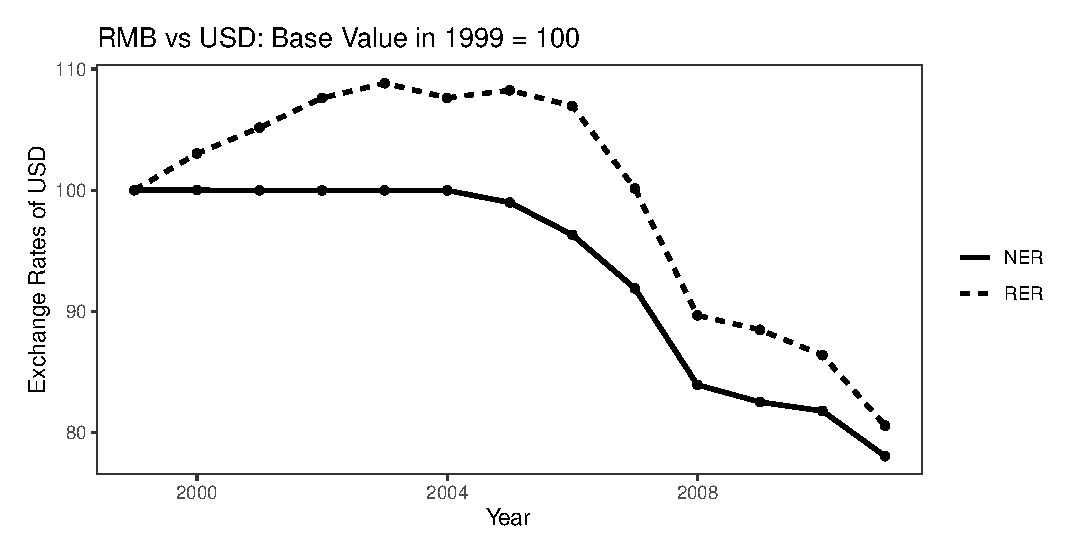
\includegraphics[width=1\textwidth]{R/USD.eps}
	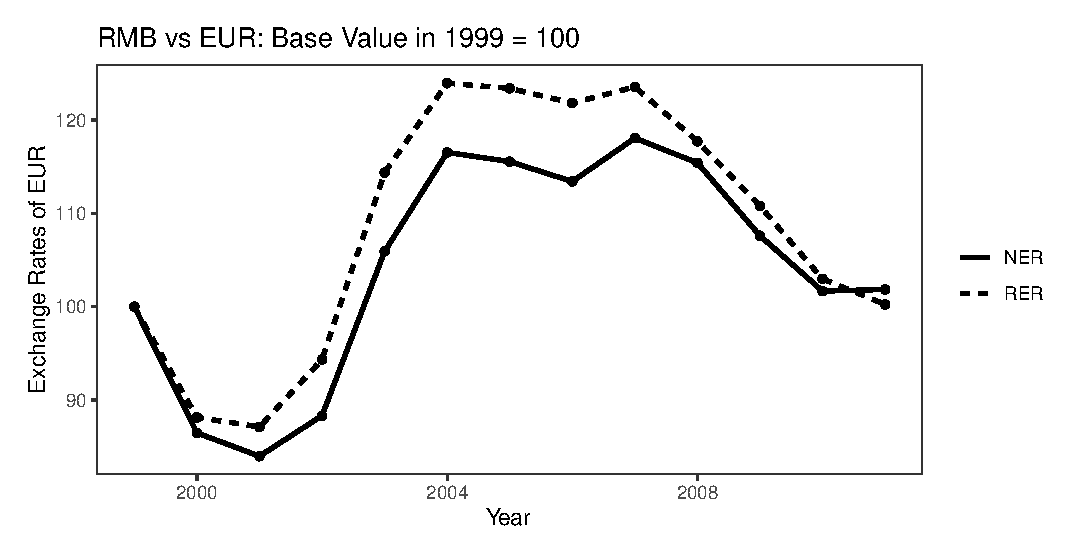
\includegraphics[width=1\textwidth]{R/EUR.eps}
	\caption{Exchange rates of Chinese RMB against USD and euro (1999-2011)}
	\label{fig.ER}
\end{figure}

\subsubsection{Customs transaction-level data} \label{Data-Customs}

We use the transaction-level records from the General Administration of Customs of China (GACC) from 2000 to 2007 for trade details.\footnote{In the original data, we have trade transactions for a longer period up to 2011, but here we only keep the sample for 2007 and before, to match the firm-level information and avoid the effects of the financial crisis.} This dataset includes the most comprehensive information on all Chinese trade transactions, including each firm's import or export value (denominated in US dollars), quantity, unit, product name and code, source or destination country, and other registration information at the customs. Using these detailed trade records, we can calculate the unit values of the firm-product pair to proxy the export and import prices.

We separate the customs records into export and import parts and focus on the latter. In our analysis, each unique transaction refers to a firm-product-country-year combination\footnote{If there are multiple import transactions by the same firm of the same product from the same country in a year, we will combine these transactions into one}. The categories of products in China's customs trade records are coded according to the Harmonized Coding and Description System (HS) of the World Customs Organization (WCO). The original data are subject to HS 8-digit classification but we aggregate HS8 product-level information to the HS6 level to make it consistent across sources.\footnote{The consolidation from HS8 to HS6 does not materially change the sample, as an importer usually buys only one HS8 product of the same HS6 category from one source, so the two are essentially equivalent.} Since there were two major revisions of the HS system in 2002 and 2007, we then use conversion tables from the United Nations Trade Statistics to convert HS 2007 and 2002 codes into the older version of HS 1996 as in \cite{fan-li-yeaple2015}. For later empirical studies, we drop incorrect or unwanted observations referring to the standard of \cite{lmx2015} \footnote{Specifically, we drop (1) products with inconsistent missing information of unit or quantity; (2) special product categories such as arms (HS2=93), antiques (HS2=97), and other special categories (HS2=98 and 99); (3) transactions existing for only one year without any change over time. These outliers make up only a small part of the observations.}.

\subsubsection{Chinese firm-level data} \label{Data-CIE}

Our source of Chinese firm-level production and financial information is the Annual Surveys of Industrial Enterprises in China (ASIE) conducted by the National Bureau of Statistics of China (NBSC). This database includes all state-owned enterprises and above-scale firms with more than 5 million Chinese RMB in annual sales. The dataset covers the period from 1999 to 2007. The number of firms each year ranged from about 130,000 in 1999 to 300,000 in 2007. The data provide details about firms’ identification codes, ownership, industry type, and about 80 other accounting variables in the balance sheet. The company information variables in this project include each firm's number of employees, total wage payment, fixed asset value, sales income, total operation input, etc. We also use firms’ registration types to categorize them as state-owned enterprises (SOEs), domestic private enterprises (DPEs), multinational firms (MNEs), and joint ventures (JVs). In later analysis, we use balance sheet variables to explore how the effect of exchange rate shocks on import prices varies with firm characteristics.

To merge these firm-level survey data with customs records, we follow the standard procedure to match identification codes based on contact information from firms as in \cite{fan-li-yeaple2015}. Manufacturing firms participating in international trade in the matched sample are uniquely identified by each observation's FRDM (legal entity) code and the survey year. We drop unsatisfactory observations referring to the criteria of \cite{bkl2021}.\footnote{We drop firms with less than ten employees and firms with incomplete information or discrepancies (e.g., negative sales or input usage). Ignoring these small-scale firms has no significant impact on our study of the pricing patterns of Chinese importing firms.} This matched sample covers the period from 2000 to 2007, and all indicators are in annual terms.

The summary statistics of the firm information dataset and the final matched sample of importers are shown in panels A and B in Table \ref{tab.summary.sample}, respectively. The notable point is that the distribution of trade value is very uneven and close to the right long-tail shape, with a few large transactions accounting for the majority of trade value. \footnote{Our finding is consistent with \cite{fan-li-yeaple2015}, in which they find the average and median firm-product-country price from 2001 to 2006 increased by 9.14\% and 13.3\%, respectively.}

\begin{table}[htbp]
        \centering
	\caption{Summary statistics for customs and firm data}
	\label{tab.summary.sample}
	\resizebox{\textwidth}{!}{
	\begin{threeparttable}
	\begin{tabular}{lcccccc}
		\toprule
             & Mean & Median & {Std. Dev} & P10 & P90 & \#observations\\
            \midrule
		\textbf{Panel A: Firm information} &       &       &       &       &       &  \\
		Sales Income (in 1000 RMB)  & 81492 & 18164 & 737089 & 5465  & 114840 & 1,619,194\\
		Employment (persons) & 256 & 106   & 939 & 30    & 491 & 1,619,194\\
		Fixed Asset (in 1000 RMB)  & 27398 & 4025  & 311063 & 572   & 36586 & 1,619,194\\
		Operation Input (in 1000 RMB)  & 63645 & 14318 & 580861 & 4143  & 90624 & 1,619,194\\
		Current wage payable (in 1000 RMB)  & 3802 & 1144  & 29502 & 278   & 6404 & 1,619,194\\
		\midrule
		\multicolumn{2}{l}{\textbf{Panel B: Matched sample with customs data}}       &       &       &       &       &  \\
  		Annual Import Price Change   & -0.0851 & -0.0018 & 1.4129 & -1.3406 &  1.1411 & 1,478,176\\
            Value per Transaction (in 1000 USD)  & 1140.97 & 14.81 & 18807.06 & 0.34 & 689.87 & 1,478,176\\
            \# Sources per Firm-product  & 2.07 & 1 & 2.27 & 1 & 4 & 1,478,176\\
		Annual Export Price Change  & 0.0248 & 0.0056 & 0.7101 & -0.5251 & 0.5940 & 1,724,591\\
            Value per Transaction (in 1000 USD)  & 786.32 & 44.08 & 17472.43 & 1.92 & 850.69 & 1,724,591\\
            \# Destinations per Firm-product  & 9.56 & 5 & 10.94 & 1 & 24 & 1,724,591\\
		\bottomrule
	\end{tabular}
	\begin{tablenotes}
        \footnotesize
	\item Notes: This table shows the summary statistics of some important variables in our major datasets. Panel A describes sales and costs information of Chinese manufacturing firms during 2000-2007. The observations in panel A are at the firm-year level. The money values in panel A are in thousands of RMB. Panel B describes the price change, the value per transaction, and the number of sources (destinations) from (to) which each firm imports (exports) a certain HS6 product for the matched sample. The observations in panel B are at the firm-product-country-year level. The money values in panel B are in thousands of USD.
	\end{tablenotes}
	\end{threeparttable}
        }
\end{table}

\subsection{Measurements of credit constraints} \label{Measurements-Credit Constraints}

An important task in our empirical strategy is to measure the extent of credit constraints. In this article, we use several proxies for sector-level financial vulnerability to measure the credit constraints faced by Chinese importers following the method of \cite{manova2013}. To deal with potential concurrent endogeneity, our measures of credit constraints are time-invariant across time. Following a widely recognized literature on the role of credit constraints in international trade (\cite{kroszner2007}; \cite{manova2013}; \cite{manova-wei-zhang2015}; \cite{fan-lai-li2015}), we use multiple financial constraint measures at the sector level to proxy for credit needs (demand for outside capital) and ability to resist financial risks. These measures are designed to reflect the nature of each industry, which should be regarded as exogenous for each firm. A firm in a more financially vulnerable industry tends to face a tighter credit constraint, regardless of its current operating conditions.

The first measure we use is external finance dependence ($ExtFin_{s}$), defined as the share of capital expenditures not financed by operational cash flows. If the degree of external finance dependence is high, the industry is more financially vulnerable, and firms in this industry are more credit-constrained. The second measure is asset tangibility ($Tang_{s}$), which describes the share of the net value of tangible assets that firms can pledge as collateral to raise external finance to its total book value. The third measure is the inventory-to-sales ratio ($Invent_{s}$), which measures the production cycle duration and the necessary working capital to maintain inventories and meet demand. 

To utilize the U.S. industry-level credit measures in the literature, we match China's CIC industry code system to the International Standard Industrial Classification (ISIC) system. We first convert 3- and 4-digit industries in the older ISIC Revision 2 from \cite{manova-wei-zhang2015} to match the newest ISIC Revision 3 codes; then we link the ISIC Revision 3 codes to the adjusted CIC codes in the CIE datasets. Finally, we match the firms in the merged sample to those sector-level financial constraint measures. For those many-to-one scenarios, when matching industry types, we assign the average value from source industries to the master industry. In this way, each Chinese firm in our sample is assigned a value for each credit measure, according to the industry in which it operates.

Although we construct three measures of credit constraints as in the literature, we will mainly focus on external finance dependence and tangibility in our later analysis. One important reason is that their interpretation can be linked to firms' exposure and resistance to financial frictions directly. On the contrary, the inventory ratio may be related to inventory management efficiency rather than liquidity and financial reasons. We also construct the first principal component of external finance dependence and asset tangibility $FPC_{s}$, which increases with the former and decreases with the latter. An industry with a higher $FPC_{s}$ is more financially sensitive in which firms require more outside funds but own less collateralizable assets. Therefore, we could use $FPC_{s}$ as an aggregate measure of financial constraints that combines information from external finance dependence and asset tangibility.

We have two reasons for using credit constraint measures based on US data in our main regressions. First, we want to remove the distortion caused by the limited credit supply in China and focus on the credit demand associated with sector-level characteristics. A nice feature of using US data to calculate credit constraint measures is that, because the US has a financially developed credit market, there is no concern that credit shortages may distort the estimation of true credit demand in an industry. Second, the U.S. patterns of sector-level credit demand are proved persistent in a cross-country setting in the literature (\cite{manova-wei-zhang2015}; \cite{fan-lai-li2015}), especially when the industry classification is broadly defined. Intuitively, the financial needs of an industry can differ in levels across countries. Still, the relative ranking between industries is supposed to be determined only by technical reasons specific to the industry itself.

Alternatively, we compute all credit measures, external finance dependence ($ExtFin_{s}$), asset tangibility ($Tang_{s}$), and inventory ratio ($Invent_{s}$) based on Chinese firm-level information from ASIE. First, we adopt the estimated value of external finance dependence from \cite{fan-lai-li2015}. Then we calculate the inventory ratio as the value of inventory over sales income, the asset tangibility as the value of fixed assets over total assets, and the R\&D intensity as R\&D spending over total sales income. To avoid endogenously affected credit constraints by other firm factors, we take the median of firm-level credit constraints among the same CIC 2-digit industry category as its industry-level credit constraint. In addition, we include the fourth measure, R\&D intensity ($RD_{s}$), defined as the ratio of research and development expenditure to the total sales, as an auxiliary measure. Usually, R\&D activities are capital-intensive, requiring firms to pay a high fixed cost before production and sales. Therefore, firms in an R\&D-intensive industry should be more financially vulnerable. However, since we only have information on firms' R\&D expenditure in and after 2005, which narrows the range of available samples, R\&D intensity will be used only as an auxiliary proxy in the robustness check. \footnote{Since the R\&D investment of many companies is equal to 0, we choose to take the average rather than the median when calculating the R\&D intensity of the industry.}

The summary statistics of the sector-level credit constraint measures in the firm-level data are shown in panel A (baseline measures calculated using the US data) and B (alternative measures calculated using the Chinese data) in Table \ref{tab.summary.credit}, respectively.
\begin{table}[H]
	\centering
	\caption{Summary statistics of measures of credit constraints}
	\label{tab.summary.credit}
	\resizebox{\textwidth}{!}{
		\begin{threeparttable}
			\begin{tabular}{lcccccc}
				\toprule
				 & \multicolumn{1}{l}{Mean} & \multicolumn{1}{l}{Median} & \multicolumn{1}{l}{Std. dev} & \multicolumn{1}{l}{P10} & \multicolumn{1}{l}{P90} & \multicolumn{1}{l}{\# Observations}\\
				\midrule
				\textbf{Panel A: US Measures} &       &       &       &       &       &  \\
				$FPC_{s}$  & 0 & 0.030 & 1.000 & -0.898  & 1.426 &  414\\
				$ExtFin_{s}$  & -0.019 & -0.040 & 0.317 & -0.22 & 0.37 & 414\\
				$Tang_{s}$  & 0.295 & 0.275 & 0.093 & 0.180 & 0.427 & 414\\
				$Invent_{s}$  & 0.164 & 0.17 & 0.032 & 0.100 & 0.196 & 414\\
				\midrule
				\textbf{Panel B: Chinese Measures} &       &       &       &       &       &  \\
				$FPC_{s}$  & -0.099 & -0.077 & 1.000 & -1.741  & 1.139 & 414\\
				$ExtFin_{s}$  & -0.643 & -0.440 & 0.664 & -1.340 & -0.100  & 414\\
				$Tang_{s}$  & 0.323 & 0.294 & 0.068 & 0.235 & 0.432 & 414\\
				$Invent_{s}$  & 0.121 & 0.117  & 0.033 & 0.083   & 0.174 & 414\\
				$R\&D_{s}$  & 0.017 & 0.014 & 0.013 & 0.007  & 0.028 & 414\\
				\bottomrule
			\end{tabular}
			\begin{tablenotes}
				\footnotesize
				\item Notes: This table shows the summary statistics of credit constraint measures. Panel A describes the measures calculated using US data, while panel B shows the alternative measures from Chinese data. $FPC_{s}$ denotes the first principal components of external finance dependence and asset tangibility. $ExtFin_{s}$ denotes external finance dependence, $Tang_{s}$ denotes asset tangibility, $Invent_{s}$ denotes inventory ratio, and $R\&D_{s}$ denotes R\&D intensity.
			\end{tablenotes}
		\end{threeparttable}
	}
\end{table}

\section{Empirical Analysis} \label{Empirical}

This section describes our empirical specifications and shows the firm–product–country-level regression results. We start from the baseline estimation of exchange rate pass-through into import prices. Then we analyze how importers' credit constraints will affect the pass-through. Finally, we will show that importers' sourcing diversity will make a difference in exchange rate pass-through for firms under different degrees of credit constraints. 

\subsection{Incomplete exchange rate pass-through into import prices} \label{Empirical-Baseline}

Past literature on firm-level evidence of exchange rate pass-through focuses on exporters' price-setting behaviors. However, importers are likely to be more than simple price takers, which gives us a new perspective on exchange rate pass-through. Therefore, we look closer at how real exchange rate fluctuations affect import prices at the detailed firm–product–country level.

Since the exchange rate pass-through is not an observable index, we need to use a panel regression to estimate it empirically. The first-step goal is to estimate exchange rate pass-through as the elasticity of unit value changes to exchange rate changes using firm-product-country observations. Referring to \cite{aik2014} and \cite{lmx2015}, we run a regression of import price changes of a certain good on the bilateral real exchange rate changes between China and its source country, controlling the change of real GDP in the source country and two-way fixed effects at firm-product-country level and year level. We view annual exchange rate changes as exogenous shocks, at least for firms. The baseline equation is shown below:

\begin{equation}
	\Delta \ln P_{i j c t}=\alpha+\beta \Delta \ln R E R_{c t}+\gamma \Delta \ln R G D P_{c t}+\xi_{i j c}+\tau_{t}+\varepsilon_{i j c t}
	\label{eq.baseline}
\end{equation}

\noindent where $P_{ijct}$ represents the import price of product $i$ bought by firm $j$ from country $c$ during year $t$. $R E R_{c t}$ is the bilateral real exchange rate between Chinese RMB and currency in the country $c$.\footnote{We also provide estimations for exchange rate pass-through into export prices to compare with past literature using the same estimation method, where import prices are replaced by export prices and the information of sources is replaced by which of destination markets.} $RGDP_{ct}$ represents the real GDP of the source country deflated to the constant price level, which proxies the market demand. $\xi_{ijc}$ denotes the firm-product-country level fixed effects to capture any time-invariant unobserved factors for a combination of firm, product, and destination. These multi-dimensional fixed effects restrict unit value changes to price adjustments rather than other product or supplier switching decisions. $\tau_t$, the time fixed effect, controls for macro-shocks that are common to all firms. We will alter the setting of those fixed effects in robustness checks.

Although prices are not directly recorded, the customs records contain disaggregated trade values (denominated by US dollars) and quantities for each HS6 product $i$, each firm $j$, from (or to) each country $c$, in each year $t$, $V_{ijct}$, and $Q_{ijct}$. We first convert the value of the goods into the local currency (RMB) using the average USD-RMB exchange rate for the year. Then, we use unit values as the proxy of import prices, defined as 

$$
P_{ijct}=\frac{V_{ijct}\times NER_{US,t}}{Q_{ijct}}
$$

\noindent where $NER_{US,t}$ is the annualized nominal exchange rate of US dollars in terms of RMB in year $t$. Because product categories are highly subdivided, we believe that the unit value is an ideal proxy for the transaction price. We will exclude observations with the annual growth rate of unit value in the top or bottom one percentile in the distribution within each HS2 product category and year group to avoid results being affected by extreme idiosyncratic factors other than exchange rate adjustments.

To deal with possible non-stationarity, we use the first difference of the logarithms for prices $\Delta \ln P_{i j c t}$, bilateral real exchange rates $\Delta \ln R E R_{c t}$ and real GDP of the source country $\Delta \ln R G D P_{c t}$ to represent their annual rates of change across years. In this way, we transform the dynamic panel into a fixed-effects regression. Therefore, using import price changes, the estimated coefficient of interest $\beta \in [0,1]$ is the elasticity of price changes to exchange rate changes (import exchange rate pass-through). Since the real prices for import $P_{i j c t}$ are denominated by the Chinese RMB in this paper, the level of coefficient $\beta$ measures the completeness of import exchange rate pass-through, i.e., a higher $\beta$ means Chinese importers face more volatile import prices denominated in Chinese RMB during exchange rate shocks.\footnote{If the $\Delta \ln P_{i j c t}$ is the export price, then the exchange rate pass-through into export prices is $1-\beta$.}

The import exchange rate pass-through estimation results are shown in column (1) of Table \ref{tab.credit} using Equation \ref{eq.baseline} with the matched sample (importers registered in the ASIE from 2000 to 2007). The average exchange rate pass-through for China in the matched sample is about 73\%. The magnitude of the coefficients means that the import prices denominated in RMB will increase by approximately 7.3\% during a 10\% real depreciation and decrease by the same amount during a 10\% appreciation. Import price fluctuations will reflect over two-thirds of exchange rate changes, while foreign currency price fluctuations will absorb the remainder. These results imply that Chinese importers must bear less than complete cost fluctuations under exchange rate shocks. 

\begin{table}[H]
	\centering
	\caption{Exchange rate pass-through to import prices and credit constraints}
        \setlength{\tabcolsep}{2mm}
	\begin{threeparttable}	
		\begin{tabular}{lccccc}
			\toprule
			& (1)   & (2)   & (3)   & (4) & (5)\\
			\midrule
                Dependent Var: & \multicolumn{5}{c}{ Import Prices $\Delta \ln P_{ijct}$} \\
			& Baseline & FPC   & External & Tangibility & Inventory \\
                & && Finance&& \\
			\midrule
			$\Delta \ln RER_{ct}$ & 0.732*** & 0.351*** & 0.493*** & 1.986*** & -0.930** \\
			& (0.075) & (0.064) & (0.065) & (0.258) & (0.420) \\
			$\Delta \ln RGDP_{ct}$ & 0.117 & 0.170 & 0.115 & 0.141 & 0.156 \\
			& (0.182) & (0.183)& (0.182) & (0.183) & (0.183) \\
			$\Delta \ln RER_{ct} \times FPC_{s}$ & &0.573*** &       &       &  \\
			& &(0.089) &       &       &  \\
			$\Delta \ln RER_{ct} \times ExtFin_{s}$ &  &  & 1.749*** &       &  \\
			& &  & (0.266) &       &  \\
			$\Delta \ln RER_{ct} \times Tang_{s}$ &   &    &   & -5.111*** &  \\
			&   &   &    & (0.960) &  \\
			$\Delta \ln RER_{ct} \times Invent_{s}$ &    &   &    &       & 9.536*** \\
			&   &    &   &       & (2.460) \\
                \midrule
			Year FE  & Yes & Yes   & Yes   & Yes   & Yes \\
			Firm-product-country FE & Yes & Yes   & Yes   & Yes   & Yes \\
			Observations & 1449210 & 1449210 & 1449210 & 1449210 & 1449210 \\
			\bottomrule
		\end{tabular}
		\begin{tablenotes}
			\footnotesize
			\item Notes: Robust standard errors clustered at firm level;  *, **, and *** indicate significance at 10\%, 5\%, and 1\% levels. Columns (2)-(5) use different measures of credit constraints calculated using U.S. data. All regressions include firm-product-country fixed effects and year fixed effects.
		\end{tablenotes}
	\end{threeparttable}
	\label{tab.credit}
\end{table}


Besides, we also show results using alternative samples of importers in Table \ref{tab.alt.imp}. Column (1) shows the import exchange rate pass-through for the whole customs sample from 2000 to 2007, including all importers that appear at least once in customs records, whether or not registered in the ASIE. Column (2) and column (3) report the pass-through among subsets of the matched sample, including only the top 50 and top 20 trading partners of China by import value. The pass-through levels in those alternative samples are slightly different than those in the baseline regression, yet the levels are of similar magnitude.

The existing estimates of short-term ERPT in the literature \citep{burstein2014international} document the extent of exchange rate pass-through at the aggregate level, which varies widely across countries and time scales. The short-term ERPT ranges from 0.2 in the US to 0.75 in Japan while the long-term ERPT ranges from 0.51 in the US to 0.97 in France. Our estimates fall within a reasonable range documented in the literature, slightly above the short-run average for the U.S. and other OECD countries. This represents a weaker bargaining power for Chinese importing firms than their developed country counterparts. In addition, the currency choice matters for ERPT. In the case of the US, \citep{gopinath2010-currency} shows that the average ERPT for transactions denominated in the local currency (USD) is 0.25 but for those denominated in other currencies is 0.95. Our results fall in between, while slightly favoring non-local currencies. We do not have detailed information on the currency in which China's imports are denominated, but anecdotal evidence suggests that most Chinese imports are denominated in US dollars, with a small portion denominated in Chinese RMB.

On the other hand, estimates of exchange rate pass-through into Chinese export prices are reported in Table \ref{tab.credit.exp}. The estimated pass-through into export prices in each column equals one minus the coefficient of $\Delta lnRER_{ct}$. The export pass-through is nearly complete at 94\% for the matched sample. That is to say, the export price in RMB adjusts very little with fluctuations in the exchange rate. The almost complete ERPT into RMB export price echoes the finding of \cite{lmx2015}. \footnote{An explanation is that most Chinese exporters are at the lower end of the value chain, where they only have narrow profit margins, leaving no room for a pricing-to-market strategy. Most Chinese exporters have no choice but to pass all exchange rate changes to their destination prices, regardless of the potential better monopolistic competition strategies.} The exchange rate-price pass-through into China's import prices is much less complete than export prices. That is to say, for Chinese firms, when the home currency (RMB) depreciates against the currencies of major trading partners, export prices denominated in the home currency will not rise significantly, but their import costs will increase more; while when the real exchange rate of the home currency appreciates, export prices in RMB will decrease only to a limited extent, and their import costs will drop by more. If we consider a typical two-way trader in China who simultaneously imports and exports from two groups of countries with strong correlations in exchange rate fluctuations, a devaluation of the home currency will reduce his unit profits. In contrast, appreciating the local currency will widen his profit margins. The asymmetric pattern of exchange rate pass-through into import and export prices will expose Chinese firms to more exchange rate risk.

\subsection{Credit constraints and exchange rate pass-through} \label{Empirical-Credit}

Imperfections in financial markets limit the optimal decision-making of trading firms, as participation in trade requires external capital. Another goal of this paper is to assess how importers with varying degrees of financial constraints absorb exchange rate fluctuations when the home currency depreciates or appreciates. Therefore, we include an interaction term for the financial constraints of sectors in the estimation. Intuitively, firms operating in those financially vulnerable industries usually have less access to enough funds to support their international trade activities; that is, they are subject to tighter credit constraints.\footnote{In this paper, we will consider credit constraints and financial constraints to be synonymous.} 

We evaluate the effects of credit constraints on the firms' price responses to exchange rate changes using the following panel regression specification:

\begin{equation}
	\Delta \ln P_{ijct}=\alpha+\beta_{1} \Delta \ln RER_{ct}+\beta_{2} \Delta \ln RER_{ct} \times FC_{s}+\gamma \Delta \ln RGDP_{ct}+\xi_{ijc}+\tau_{t} +\varepsilon_{ijct}
	\label{eq.credit}
\end{equation}

\noindent where $FC_{s}$ represents the degree of financial (credit) constraints of the sector $s$ to which the firm $j$ belongs and the rest are the same as in the baseline equation. The interaction coefficient $\beta_2$ represents the effect of credit constraints on exchange rate pass-through. A positive $\beta_2$ for importers implies more credit-constrained importers have a more complete import exchange rate pass-through. The overall ERPT into import prices $j$ is given by $\beta_{1} +\beta^{Import}_{2} FC_{s}$. \footnote{For exporters, it is the opposite: a negative $\beta^{Export}_2$ implies more credit-constrained exporters have a complete exchange rate pass-through, and the ERPT into export prices is $1-(\beta_{1} +\beta^{Export}_{2} FC_{s})$.}

Using this estimation strategy, we hope to scrutinize how the pricing behavior of Chinese importers in response to the exchange rate is affected by credit constraints and compare it with that of exporters. While credit-constrained exporters’ pricing decisions to deal with exchange rate shocks are mainly related to production and profit margin, the penetration effect of credit constraints on import prices is through the shortage of cash or liquid funds to afford the transaction. In turn, these constraints will affect importer sourcing choices and bargaining power. According to our hypothesis in which financially more constrained firms have to take more risks, we expect that the interaction coefficients on $FPC_{s}$, $ExtFin_{s}$, and $Invent_{s}$ are negative, while the coefficient on $Tang_{s}$ is positive.

Columns (2)-(5) in Table \ref{tab.credit} present differences in exchange rate pass-through into import prices resulting from the industry-level credit heterogeneity.\footnote{Table \ref{tab.credit.exp} reports the results of the comparison for the export side.} Concerning our focus, a positive cross-term coefficient $\beta_2$ implies that the magnitude of this variable is positively related to the completeness of exchange rate pass-through. Using the first principal component of external finance dependence and asset tangibility $FPC_{s}$ to measure financial constraints $FC_{s}$, we see that import exchange rate pass-through is more complete in financially more vulnerable sectors than in financially less vulnerable sectors. Columns (3) and (4) separately show the effects of external finance dependence and asset tangibility on importers' exchange rate pass-through. Consistent with the definition that a higher degree of external finance dependence implies tighter credit constraints faced by firms, we observe a positive coefficient of $\beta_2$, which means exchange rate pass-through into prices will be more complete. In contrast, a higher degree of asset tangibility (more collateralizable assets) can alleviate financial constraints. Therefore, we observe a negative coefficient for the latter. With the auxiliary measure, the inventory ratio $Invent_{s}$, we further observe the positive effect on exchange rate pass-through in column (5). In general, the coefficients $\beta^{Import}_2$ of the interaction term $\Delta \ln RER_{ct} \times FC_{s}$ of all measures are positive and significant at the 1\% level. 

Our evidence supports the hypothesis that exchange rate fluctuations are more likely to be reflected in unstable import costs for importers in more financially vulnerable industries because they have weak bargaining power in the international trade market. External financing dependence, internal collateral capacity, and inventory turnover act both jointly and separately on the exchange rate pass-through of importers. Inadequate funding results in limited financial flexibility for these importers. They might not be able to negotiate better deals or absorb unexpected costs. This situation puts them in a weaker bargaining position compared to buyers who have more market power. When sellers have more market power, they can dictate terms and conditions to importers. Importers under tight credit constraints are less able to absorb these cost changes due to their limited financial capacity. As a result, sellers will force the financially constrained importers to bear the brunt of the exchange rate fluctuations. This dynamic illustrates how importers' credit constraints will affect the pass-through of exchange rates into import prices through buyers' market power.

It is worth noting that the exchange rate pass-through here is estimated by the at-the-dock import price in our specification. This excludes any impact of credit constraints on post-landing costs, such as local distribution and logistics costs. In other words, the impact of credit constraints on import costs found here works mainly by affecting the supplier's pricing behavior. Since buyers' characteristics cannot influence sellers' marginal costs, import price pass-through is almost entirely determined by sellers' markups. If the seller's markup is rather more fixed, then the exchange rate pass-through is more complete. Intuitively, firms in more credit-constrained industries may have weaker import bargaining power, and product prices are more likely to be pegged to the US dollar (vehicle currency pricing, VCP) or the currency of the exporting country (producer currency pricing, PCP, less pricing-to-market), so at-the-dock prices respond more to exchange rate fluctuations regardless of any domestic market factor.

In addition, we can derive comparative results on the effect of credit constraints on pass-through into export prices as in columns (2)-(5) in Table \ref{tab.credit.exp}. The estimates suggest that financial constraints lead export exchange rate pass-through to a more complete degree, although the initial ERPT is already nearly complete. These results are consistent with the finding of \cite{strasser2013}, who argues that financially constrained firms have higher export price pass-through than unconstrained firms. Credit constraints restrict exporters from absorbing exchange rate shocks, potentially because firms need external finance to apply pricing-to-market strategies in foreign markets. Although the import ERPT is significantly less complete than the export ERPT, we can still conclude that credit constraints steer import pass-through toward a more complete degree. Manufacturing firms with a more vulnerable credit condition will have much more volatile imported intermediate costs. For credit-constrained two-way traders, given that import sources and export markets cannot be adjusted quickly, the unit profit margin is more sensitive to exchange rate fluctuations. Therefore, credit constraints expose Chinese manufacturing firms to greater exchange rate risks in international trade.

Nonetheless, while the direction in which credit constraints affect the exchange rate pass-through on the export and import sides is the same, underlying channels may be different. A higher external finance premium causes higher marginal costs, so firms with binding financial constraints have no choice but to set higher prices and face a higher price elasticity of demand. When there is an exchange rate shock, the optimal choice is to adjust their markups, but credit-constrained firms can do so only to a limited extent because they have narrower profit margins. However, for import pass-through, credit constraints affect how buyers pay in the transactions. Adequate credit or cash reserves give importers strong bargaining power, for example, by allowing them to negotiate a longer-term (or with more stable prices) purchase agreement, where foreign sellers will bear more exchange rate fluctuations. In this way, a financially ``weaker'' importer may not have the buffer to transfer any risk, so it must pay immediately and accept current exchange rate settlements, which means taking on more volatile prices.

\subsection{Sourcing diversity and credit constraints}

After estimating exchange rate pass-through at the firm level and the effect of credit constraints, we need to go a step further to explore the mechanism. Through what channels do credit constraints affect the ability of importers to cope with exchange rate shocks? What other factors related to a firm's sourcing power would exacerbate or diminish this effect? Are the effects of credit constraints fully explained by these factors? To answer the questions, we add a vector $\mathbb{Z}_{jt}$ to include additional factors and apply it to control terms and the interaction terms with real exchange rate changes:\footnote{We will also use its lagged form $\mathbb{Z}_{jt-1}$, the initial time value $\mathbb{Z}_{jt_0}$ or mean level $\bar{\mathbb{Z}}_{jt}$ to eliminate possible simultaneous endogeneity in the robustness check.} 

\begin{equation}
    \begin{aligned}
    \Delta \ln P_{ijct}=&\alpha+[\beta_{1}+ \beta_{2} \times FC_{s}+\beta_{3} \times {\mathbb{Z}_{jt}}'] \Delta \ln RER_{ct} \\ &+\gamma \Delta \ln RGDP_{ct}+ {\mathbb{Z}_{jt}}' \eta+\xi_{ijc}+\tau_{t} +\varepsilon_{ijct}.
    \end{aligned}
    \label{eq.add.control}
\end{equation}

\begin{equation}
    \begin{aligned}
    \Delta \ln P_{ijct}=&\alpha+[\beta_{1}+ \beta_{2} \times FC_{s}+\beta_{3} \times {\mathbb{Z}_{jt}}'+\beta_{4} \times FC_{s} \times {\mathbb{Z}_{jt}}'] \Delta \ln RER_{ct} \\ &+\gamma \Delta \ln RGDP_{ct}+ {\mathbb{Z}_{jt}}' \eta+\xi_{ijc}+\tau_{t} +\varepsilon_{ijct}.
    \end{aligned}	
    \label{eq.add.interaction}
\end{equation}

With the estimation strategy in the form of Equation \ref{eq.add.control} and Equation \ref{eq.add.interaction}, we can analyze various factors that may directly or indirectly affect exchange rate pass-through. The coefficient of the interaction term between additional factors and real exchange rate movement $\beta_3$ represents the direct effects of those factors on the exchange rate pass-through other than financial constraints. In Equation \ref{eq.add.interaction}, the triple interaction coefficient $\beta_4$ represents the indirect effects of these factors on the pass-through of the exchange rate through financial constraints. The same sign of $\beta_4$ and $\beta_2$ means that this additional factor improves the effect of credit constraints, while the opposite sign means it alleviates the effect of credit constraints.

In the face of exchange rate shocks, firms are at risk of import price volatility and will try to stabilize their imports to avoid production disruptions due to input shortages. Diversification of import linkages will help firms maintain more resilient supply relationships. An intuitive explanation for this is that it is more costly for firms to find new suppliers in countries they have never entered before, whereas it is cheaper to increase imports from suppliers with whom they already have a relationship or to purchase from new suppliers in countries where they already have sourcing experience. Firms sourcing from only a few countries are more exposed to exchange rate shocks than firms sourcing in a decentralized manner.
Firms sourcing from only a few countries are more exposed to exchange rate shocks than firms that diversify their sourcing. In this part, we will examine how sourcing diversity affects exchange rate pass-through for firms subject to different levels of credit constraints.

Following the literature, an importer's sourcing diversity could increase its bargaining power in import prices in addition to its production characteristics. We argue that the more diverse a firm's sourcing choices are, the more flexible it is in adjusting its import sources when facing shocks. If a firm can respond to shocks by adjusting its supply network more flexibly, its uncertainty about cost prices should diminish. Therefore, a potential mechanism through which financial constraints affect an importer's bargaining power with foreign suppliers is its outside sourcing options. Companies with more trading partners can flexibly switch to another supplier or adjust the weight of imports from different countries. Firms with heterogeneous sourcing capacity may therefore be affected by credit constraints to a different extent. 

We want to test how importers' sourcing diversity affects exchange rate pass-through. First, we will use the number of source countries $Source_{ijt}$ from which an importer $j$ imports a certain type of HS6 product $i$ in year $t$ to measure the firm-product level sourcing diversity. We employ Equation \ref{eq.add.interaction} that includes the number of import sources for each firm-product pair. The estimation results of sourcing diversity are reported in Table \ref{tab.source}.

\begin{sidewaystable}[htbp]
	\centering
	\caption{Import sources, credit constraints, and exchange rate pass-through}
	\resizebox{\textwidth}{!}{
	\begin{threeparttable}
		\begin{tabular}{lcccccccc}
			\toprule
			& (1)   & (2)   & (3)   & (4) & (5)   & (6)   & (7)   & (8)   \\
			\midrule
                Dependent Var: & \multicolumn{8}{c}{ Import Prices $\Delta \ln P_{ijct}$} \\
			 & \multicolumn{4}{c}{Current Sources} & \multicolumn{4}{c}{Initial Sources} \\
			& \#Sources & \#Sources+ & \#Sources+ & \#Sources+	& \#Sources & \#Sources+ & \#Sources+ & \#Sources+ \\
			&       & FPC &External & Tangibility &  & FPC &External & Tangibility\\
			&       & &Finance & &       & &Finance &			\\
			\midrule
			$\Delta \ln RER_{ct}$ & 0.950*** & 0.550*** & 0.696*** & 2.375*** & 0.930*** & 0.548*** & 0.683*** & 2.282*** \\
			& (0.055) & (0.058) & (0.054) & (0.146) & (0.054) & (0.059) & (0.054) & (0.147) \\
			$\Delta \ln RGDP_{ct}$ & 0.143 & 0.080 & 0.080 & 0.108 & 0.143 & 0.082 & 0.082 & 0.109 \\
			& (0.126) & (0.126) & (0.126) & (0.126) & (0.126) & (0.126) & (0.126) & (0.126) \\
			$\Delta \ln RER_{ct} \times \#Source_{ijt}$ & -0.059*** & -0.059*** & -0.057*** & -0.081*** & -0.066*** & -0.071*** & -0.065*** & -0.076*** \\
			& (0.009) & (0.010) & (0.009) & (0.024) & (0.010) & (0.012) & (0.010) & (0.028) \\
			$\Delta \ln RER_{ct} \times FPC_{s} \times \#Source_{ijt}$ &    & -0.015** &       &       &       & -0.011 &       &  \\
			&   & (0.007) &       &       &       & (0.009) &       &  \\
			$\Delta \ln RER_{ct} \times FPC_{s}$ &  & 0.670*** &       &       &       & 0.637*** &       &  \\
			&   & (0.046) &       &       &       & (0.047) &       &  \\
			$\Delta \ln RER_{ct} \times ExtFin_{s} \times \#Source_{ijt}$ &   &       & -0.064*** &       &       &       & -0.058** &  \\
			&   &       & (0.020) &       &       &       & (0.025) &  \\
			$\Delta \ln RER_{ct} \times ExtFin_{s}$ &     &       & 2.113*** &       &       &       & 2.024*** &  \\
			&   &       & (0.137) &       &       &       & (0.140) &  \\
			$\Delta \ln RER_{ct} \times Tang_{s} \times \#Source_{ijt}$ &    &       &       & 0.049 &       &       &       & -0.005 \\
			&    &       &       & (0.098) &       &       &       & (0.116) \\
			$\Delta \ln RER_{ct} \times Tang_{s}$ &   &       &       & -5.665*** &       &       &       & -5.374*** \\
			&  &       &       & (0.537) &       &       &       & (0.552) \\
                \midrule
			Year FE  & Yes   & Yes   & Yes   & Yes & Yes   & Yes   & Yes   & Yes\\
			Firm-product-country FE & Yes   & Yes   & Yes   & Yes & Yes   & Yes   & Yes   & Yes\\
			Observations & 1449210 & 1449210 & 1449210 & 1449210 & 1449210 & 1449210 & 1449210 & 1449210\\
			\bottomrule
		\end{tabular}
		\begin{tablenotes}
			\footnotesize
			\item Notes: Robust standard errors clustered at firm-product level; *, **, and *** indicate significance at 10\%, 5\%, and 1\% levels. Columns (1)-(4) use the number of source countries in the current year, while columns (5)-(8) use the number of source countries in the initial year. All regressions include firm-product-country fixed effects and year fixed effects.
		\end{tablenotes}
	\end{threeparttable}
	}
	\label{tab.source}
\end{sidewaystable}

The estimates for intersection terms between import sources and real exchange rate changes are shown in column (1). We find that an importer who imports a certain product from more sources will have a less complete pass-through. This is consistent with our hypothesis that importers with more alternative sourcing options will have less complete pass-through. In other words, the diversity of import sources for the same product can significantly enhance the stability of import prices. After adding interactions, we find the effects of credit constraints still exist while the triple interaction terms with the number of sources have the opposite while still significant coefficients in columns (2) and (3). The triple interaction term in column (4) is not significant, probably because the offsetting effect of sourcing diversity is mainly for industries that are more dependent on external financing than weaker collateralization capabilities. Columns (5)-(8) repeat the above test using the number of source countries in the initial year (the year in which the firm appeared for the first time in this sample) as the measure of sourcing diversity to deal with possible simultaneous endogeneity problems. Since our fixed effects include firm-product combinations, we have already excluded the effect of firm size on the demand for the specific product.

In Appendix Table \ref{tab.source.distance}, we will use geographical distances as alternative measures of import sources. Intuitively, firms that can import a certain good from more distant countries generally have greater sourcing power because they can afford the cost of transportation over long distances. Those firms should also be able to choose from more diversification options during shocks. We, therefore, consider product-specific distances as another indicator of sourcing diversity. We used straight-line distances between the most populated cities (simple distances), and population distribution-weighted distances as measures of trade distance, and the results remained consistent. As we expected, the results using geographic distance and the results using the number of sources are nearly identical in terms of the sign and significance of the coefficients.

The results show that a wider sourcing base will mitigate the effects of credit constraints and their direct effects on exchange pass-through into import prices. The opposing effects of credit constraints and sourcing diversity on exchange rate pass-through confirm the existence of the bargaining power of importers. We show that if a firm can import the same product from more sources, even if it operates in a financially demanding industry, it can utilize its alternative options to escape the unfavorable bilateral exchange rate risk from a certain source country. The firm with a more diverse sourcing network can either switch from one supplier to another to reduce its input costs (i.e., trade diversion effect) or make a more credible threat to negotiate a more stable price. Therefore, firms with more import sources will be better cushioned against fluctuations in the cost of imported inputs due to changes in exchange rates.

\section{Robustness} \label{Robustness}

In this chapter, we provide a series of additional robustness checks to confirm our empirical findings. First, we use alternative measures of credit constraints computing from Chinese data instead of from U.S. data. Second, we exclude countries whose fiat currency is the US dollar or is pegged to the US dollar. Third, we control importers' trade modes in two dimensions: ``two-way trade'' and ``processing trade''. Fourth, we control the ownership and affiliation types of importers. Fifth, we control revenue-based estimated firm-level markups. Finally, we use alternative estimation methods. All test results indicate that our findings are robust.

\subsection{Alternative measures of credit constraints}

As all results in the baseline regression use the credit constraint measures based on US data, here we use alternative credit constraint measures using Chinese firm data to verify our baseline results. The purpose is to avoid potential bias from differences in the attributes of industry credit demand in different countries. The details of constructing these Chinese variables are discussed in Section \ref{Measurements-Credit Constraints}. Although China's financial markets are less mature than the U.S., the relative rankings of the degree of credit constraint in different sectors are similar \citep{manova2013}. Therefore, the credit constraint measures calculated based on Chinese data are expected to be consistent with the main findings. 

Our results are reported in Table \ref{tab.robust.credit}, which can be easily compared with the results using US measures. Columns (1)-(4) of Table \ref{tab.robust.credit} present the effects of external finance dependence, tangibility, inventory ratio, and R\&D intensity on exchange rate pass-through into import prices, respectively. Nevertheless, all interaction term coefficients exhibit the same signs and significance as above, confirming the validity of the effects of credit constraints on the exchange rate pass-through shown in the previous section. Even column (4) using the auxiliary measure R\&D intensity shows that firms in industries with greater R\&D investment also have more complete exchange rate pass-through. With alternative measures calculated using Chinese data, we can conclude that financially more constrained importers have more complete exchange rate pass-through into prices than those less constrained.

\begin{table}[H]
	\centering
	\caption{Robustness check: alternative credit constraints measures from Chinese data}
        \resizebox{\columnwidth}{!}{
	\begin{threeparttable}
	\begin{tabular}{lccccc}
		\toprule
		& (1)   & (2)   & (3)   & (4) \\
		\midrule
            Dependent Var: & \multicolumn{4}{c}{ Import Prices $\Delta \ln P_{ijct}$} \\
		& \multicolumn{4}{c}{Measures of Credit Constraints from Chinese Data} \\
		  & External Finance & Tangibility & Inventory & R\&D Intensity \\
		\midrule
		$\Delta \ln RER_{ct}$  & 0.943*** & 3.427*** & -0.966*** & 0.215* \\
		 & (0.113) & (0.395) & (0.267) & (0.110) \\
		$\Delta \ln RGDP_{ct}$  & 0.154 & 0.142 & 0.168 & 0.160 \\
		 & (0.183) & (0.182) & (0.183) & (0.183) \\
		$\Delta \ln RER_{ct} \times ExtFin_{s}$ & 0.327** &       &       &  \\
		& (0.134) &       &       &  \\
		$\Delta \ln RER_{ct} \times Tang_{s}$ &        & -9.321*** &       &  \\
		&   &   (1.286) &       &  \\
		$\Delta \ln RER_{ct} \times Invent_{s}$ &           &       & 14.919*** &  \\
		&       &       & (2.433) &  \\
		$\Delta \ln RER_{ct} \times R\&D_{s}$ &         &       &       & 26.607*** \\
		&         &       &       & (5.291) \\
            \midrule
		Year FE  & Yes   & Yes   & Yes & Yes \\
		Firm-product-country FE   & Yes   & Yes   & Yes & Yes\\
		Observations & 1449210 & 1449210 & 1449210 & 1449210 \\
		\bottomrule
	\end{tabular}
	\begin{tablenotes}
		\footnotesize
		\item Notes: Robust standard errors clustered at firm level; *, **, and *** indicate significance at 10\%, 5\%, and 1\% levels. The dependent variable is the price change $\Delta \ln P_{ijct}$. Columns (1)-(4) use different measures of credit constraints calculated using Chinese data. All regressions include firm-product-country fixed effects and year fixed effects.
	\end{tablenotes}
	\end{threeparttable}
        }
        \label{tab.robust.credit}
\end{table}

\subsection{Excluding the dollar peg effect}

From 1994 until July 2005, the People's Bank of China pegged the Chinese yuan (RMB) to the US dollar. This policy regime has kept the Chinese RMB undervalued persistently. The effect on trade is that China's exports are cheaper in terms of foreign currency and, therefore, more attractive than those of other countries. Due to China's exchange rate peg to the US dollar, we observe weak movements in the nominal exchange rate of RMB against the USD and other currencies pegged to the US dollar until 2005, as shown in Figure \ref{fig.ER}. During this period, estimates of the elasticity of import prices to exchange rate changes may be inaccurate if including the RMB-USD exchange rate peg.

We will perform robustness tests using an alternative sample to eliminate the confounding effect of the RMB-USD exchange rate peg on import pass-through. Specifically, we exclude the U.S. and other countries that use the US dollar as their official currency or whose currency is pegged to the US dollar from our sample.\footnote{The excluded countries and regions using the US dollar or pegging to the US dollar are Belize, Liberia, Qatar, Ecuador, Djibouti, Saint Lucia, Saint Kitts and Nevis, St. Vincent, and the Grenadines, Dominica, Antigua and Barbuda, Palestine, Bahamas, Barbados, Panama, Bahrain, Curaçao, Grenada, Saudi Arabia, Zimbabwe, Macao SAR of China, Turks and Caicos Islands, Bermuda, Jordan, United States, British Virgin Islands, Dutch Sint Maarten, El Salvador, Montserrat, United Arab Emirates, Oman, Aruba, Hong Kong SAR of China, Maldives, Lebanon.}. We examine whether our previous conclusion is robust after excluding those countries whose currencies are denominated in or pegged to the US dollar.

\begin{table}[H]
	\centering
	\caption{Robustness check: alternative samples excluding countries using USD or USD-pegged currencies}
	\begin{threeparttable}
	\begin{tabular}{lcccc}
		\toprule
		& (1)   & (2)   & (3)   & (4) \\
		\midrule
            Dependent Var: & \multicolumn{4}{c}{ Import Prices $\Delta \ln P_{ijct}$} \\
		& \multicolumn{4}{c}{Excluding US Dollar Peg} \\
		& Baseline & FPC   & External Finance & Tangibility \\
		\midrule
		$\Delta \ln RER_{ct}$ & 0.849*** & 0.511*** & 0.642*** & 2.021*** \\
		& (0.086) & (0.086) & (0.081) & (0.266) \\
		$\Delta \ln RGDP_{ct}$ & 0.770*** & 0.678*** & 0.686*** & 0.710*** \\
		& (0.252) & (0.247) & (0.247) & (0.249) \\
		$\Delta \ln RER_{ct} \times FPC_{s}$ &    & 0.526*** &       &  \\
            & & (0.086) &       &  \\
		$\Delta \ln RER_{ct} \times ExtFin_{s}$ & &       & 1.590*** &  \\
		& &       & (0.255) &  \\
		$\Delta \ln RER_{ct} \times Tang_{s}$ & &       &       & -4.753*** \\
		& &       &       & (0.933) \\
            \midrule
		Year FE  &   Yes    & Yes   & Yes   & Yes \\
		Firm-product-country FE &   Yes    & Yes   & Yes   & Yes \\
		Observations & 1147027 & 1147027 & 1147027 & 1147027 \\
		\bottomrule
	\end{tabular}
	\begin{tablenotes}
		\footnotesize
		\item Notes: Robust standard errors clustered at firm level; *, **, and *** indicate significance at 10\%, 5\%, and, 1\% levels. We exclude countries that use the U.S. dollar or currencies pegged to the U.S. dollar. Columns (2)-(4) use different measures of credit constraints calculated using U.S. data. All regressions include firm-product-country fixed effects and year fixed effects.
	\end{tablenotes}
        \end{threeparttable}
        \label{tab.robust.nopeg}
\end{table}

Table \ref{tab.robust.nopeg} demonstrates that our results excluding the U.S. and those pegged countries are not overturned. The estimated import ERPT from the rest of the world other than USD-pegged countries is 84.9\% in column (1), slightly more complete than 73.2\% in the matched sample. All coefficients on interaction terms remain robust and significant, suggesting that higher external finance dependence makes exchange rate pass-through more complete, while higher asset tangibility plays the opposite role. Therefore, the nominal peg of RMB to the dollar before 2005 does not interfere with the main conclusions of this paper.

\subsection{Trade type controls}

We acknowledge that manufacturing firms participating in trade involve different types of trade. We will perform two groups of tests to control different trade modes in our estimates of exchange rate pass-through.

First, some importers may purchase goods from foreign suppliers while others may be ``two-way traders'' who export and import within the same year. Simultaneous exports and imports could interact with each other and affect their exchange rate pass-through. Specifically, exporting importers may pass part of the price fluctuations of imported intermediate goods caused by exchange rate shocks to their export destination to hedge the exchange rate risk. To test whether our results about credit constraints and exchange pass-through change after considering this two-way effect, we include a ``two-way'' indicator as our control, which takes the value of 1 when a company imports or exports simultaneously and 0 when it only imports.

Second, some importers may be registered as ``processing trade'', who sign contracts with foreign customers to import raw materials and intermediate inputs from those customers by credit for domestic processing and re-export (\cite{manova-yu2016}). Economists usually believe that processing-trade firms may behave differently from other firms in their trading behaviors. Ordinary trade accounts for more than 2/3 of the total transactions in our sample. Therefore, the pricing patterns based on ordinary trade should dominate the overall Chinese trade. However, being cautious about the effect of credit constraints on exchange rate pass-through concerning processing trade, we control its trade mode in the robustness checks, which take the value of 1 when a transaction belongs to ordinary trade and 0 when it belongs to processing trade.

Table \ref{tab.robust.tradetype} shows that the results after controlling for two-way trade and processing trade are very similar to those of the matched sample. Although firms do actively choose different trade modes based on their capabilities, these differences do not affect our main conclusions on credit constraints and ERPT.

\subsection{Firm ownership controls}

Sector-level financial variables have the important advantage of being exogenous. However, firms are likely to have heterogeneous credit conditions even within a narrowly defined sector. An important feature of the financing environment in China is that the connection to company owners and its ease of access to credit are highly correlated. Therefore, firm ownership may be another potential factor affecting credit constraints, as importers can obtain additional credit support from their parent firms or owners to finance a larger share of extra costs into international trade. Given the underdevelopment of Chinese financial markets, firms with different types of ownership are likely to have different credit access in addition to their heterogeneous credit demand based on industry characteristics. 

Therefore, we add ownership information as additional controls of firm characteristics into the estimations of exchange rate pass-through to check our main results. Specifically, we will use two different ownership classification criteria. First, we use the 3-digit registration type codes in the ASIE. We grouped these different registration codes into four large categories: state-owned enterprises (SOE), domestic private enterprises (DPE), multinational enterprises (MNE), and joint ventures (JV), among which we take DPE as our default group. Second, we will assign an ``affiliation'' indicator for each importer using matching correspondence data between parent firms and subsidiaries, which takes the value of 1 when an importer is not a subsidiary of another company and takes 0 and vice versa. We use the dummy to control the impact of affiliation on firm-level credit access.

Table \ref{tab.robust.ownership} in the Appendix shows the results after controlling for different ownership types.\footnote{Since a firm's registration type is almost time-invariant, we cannot include firm-product-country fixed effects when using the registration type control. Therefore, we use the combination of product-country fixed effects and sales income control to replace firm-product-country FE in our specification.} The signs and significance of regression coefficients for all types of firms are the same as in the previous main results. This suggests that although ownership type may cause differences among firms, the impact of sector-level credit constraints on exchange rate pass-through cannot be ignored among importers.

\subsection{Markup controls}

We have argued that credit constraints will affect the ``absorptive capacity'' of exchange rate shocks. Referring to previous studies on exchange rate pass-through to export prices, firms with various levels of markup have the heterogeneous ability to pass on fluctuations in the exchange rate to the export market \citep{aik2019}. From the fact that ``big sellers are also big buyers'' \citep{aik2014}, we want to check whether our arguments for credit constraints and exchange rate pass-through into import prices still hold after controlling for firm-level markups.

On the one hand, for two-way traders, export prices could act as a ``pressure-reducing valve'' for import costs. A firm that can pass more exchange rate fluctuations to destination prices has more room to absorb price fluctuations of imported inputs. In this way, the export and import prices of the same firm will be positively correlated under shocks. On the other hand, advantages in a firm's competitiveness, either explicit ones shown in its markup or productivity or implicit ones like foreign networks, may lead to greater bargaining power in the trade market and thus cause less complete price pass-through into both export and import prices.

Our firm-level data contains production information so that we can connect the exchange rate pass-through with estimated firm-specific markup. In this part, we will control markups to check our arguments. Following \cite{bkl2021}, we can estimate the firm-level markup without direct prices and marginal cost measures using the structural assumptions of \cite{dlw2012} and the GMM estimation method. Specifically, we derive the firm-specific markup as the ratio of an input factor's output elasticity to its firm-specific factor payment share $\mu_{t}=\theta_{t}^{X}\left(\alpha_{t}^{X}\right)^{-1}$, where $\alpha_{t}^{X}$ is the share of expenditures on input X in total sales and $\theta^X_t$ denotes the output elasticity on input X. We apply the methodology of \cite{acf2015} to calculate the firm-specific output elasticity concerning materials using estimated firm-specific production functions, assuming a 3rd-order translog gross output production function in capital $k$, labor $l$, and material inputs $m$ in the form of: $ y_{t}= \beta_{k} k_{t}+\beta_{l} l_{t}+\beta_{i} m_{t}+\beta_{k 2} k_{t}^{2}+\beta_{l 2} l_{t}^{2}+\beta_{m 2} m_{t}^{2}+ \beta_{k l} k_{ t} l_{t}+\beta_{k m} k_{t} m_{t}+\beta_{l m} l_{t} m_{t}+\beta_{k 3} k_{t}^{3}+\cdots+\omega_{t}+\epsilon_{t}.
$\footnote{In practice, we construct four production variables in logarithmic form: real output value $y_t$, persons engaged $l_t$, real fixed assets at current value $k_t$, and real material inputs $m_t$. Output values are deflated by output deflators, while fixed assets and material inputs are deflated by investment deflators and input deflators. The deflators are constructed as in \cite{brandt2012}.}

In the literature, firms with different sales markups have heterogeneous responses to exchange rate shocks. The same logic may also apply to import exchange rate pass-through. \cite{llz2018} provide micro evidence that internal finance and external credit supply significantly promote firms' sales growth rates. Now we add estimated firm-level markup into interactions, and the results are shown in Table \ref{tab.markup}: the effects of credit constraints on exchange rate pass-through are significant after controlling for importers' revenue-based markups. This indicates that markup cannot fully explain the effect of credit constraints, which is consistent with the finding in \cite{xu-guo2021}.

However, the explanation for import-side absorptive capacity is more complicated than for exporters' markup. \cite{bmm2012} documents that more productive firms react to depreciation or appreciation by adjusting more markups and less export volume, keeping local market prices relatively stable (less complete pass-through). This explanation hinges on endogenous markups over marginal costs, where less elastic demand allows more extensive markup adjustments during exchange rate shocks. However, on the import side, other factors concerning sourcing capacity and buyers' market power also play a remarkable role in exchange rate pass-through. In any case, the effects of credit constraints on import prices are not offset or replaced by seller-side markups.

\subsection{Alternative estimation methods}

Our estimation strategy includes multiple data dimensions, including product, source country, and time. Therefore, the baseline estimation of exchange rate pass-through adapts panel fixed-effects regression, in which $\xi_{ijc}$, the firm-product-country level three-dimensional fixed effects and $\tau_t$, the time fixed effects, thereby lead to accurate estimation of price changes only due to exchange rate shocks. In this section, we will try alternative estimation methods to check the robustness of our results.

First, we will check whether other fixed-effect combinations yield similar results. In baseline specifications, we do not have perfect controls for all firm-year covariates. In the following tests, we will combine firm-year fixed effects $\tilde{\xi}_{jt}$ with two-dimensional product-country fixed effects $\lambda_{ic}$ as in Equation \ref{eq.credit.fe1} or separately with product fixed effects $\lambda_{1, i}$ and country fixed effects $\lambda_{2, c}$ as in Equation \ref{eq.credit.fe2}. The results of alternative combinations of fixed effects are shown in columns (1)-(4) and (5)-(8) in Table \ref{tab.robust.fe}, respectively. 

\begin{equation}
    \Delta \ln P_{ijct}=\alpha+\beta_{1} \Delta \ln RER_{ct}+\beta_{2} \Delta \ln RER_{ct} \times FC_{s}+\gamma \Delta \ln RGDP_{ct}+\tilde{\xi}_{jt}+\lambda_{ic}+\varepsilon_{ijct}
	\label{eq.credit.fe1}
\end{equation}

\begin{equation}
    \Delta \ln P_{ijct}=\alpha+\beta_{1} \Delta \ln RER_{ct}+\beta_{2} \Delta \ln RER_{ct} \times FC_{s}+\gamma \Delta \ln RGDP_{ct}+\tilde{\xi}_{jt}+\lambda^1_{i} + \lambda^2_{c} +\varepsilon_{ijct}
	\label{eq.credit.fe2}
\end{equation}

Second, to avoid firm endogeneity, our measures of credit constraints only capture the cross-sectional pattern, i.e., the industry-level credit needs measures are persistent and thus averaged over time. Therefore, to fully sort out the time variation effect, we also conduct cross-sectional estimation using both a one-year sample and between estimators\footnote{The between estimator with bars indicate average variables and therefore the time variation has been averaged out.}, with the following equation:

\begin{equation}
	\overline{\Delta \ln P}_{ijc}=\alpha+\beta_{1} \overline{\Delta \ln RER}_{c}+\beta_{2} \overline{\Delta \ln RER}_{c} \times FC_{s}+\gamma \overline{\Delta \ln RGDP}_{c}+\bar{\xi}_{ij} +\varepsilon_{ijc}
	\label{eq.credit.crosec}
\end{equation}

In Table \ref{tab.robust.crosec} in the Appendix, we report the one-year results using the subsample in the last year 2007\footnote{The year 2007 is randomly picked in the sample period, and the results with other years are not shown here but are available upon request.} in columns (1)-(4) and the between estimator results averaging the price changes and real exchange rate changes in columns (5)-(8). All the results on the estimated ERPT into import prices and the effect of credit constraints are similar to previous findings on the effects of credit constraints on ERPT.

\section{Discussions} \label{Discussion}

In this section, we further investigate the heterogeneity of firms in import bargaining power and its impacts on firms’ responses to exchange rate movements. Although our results and robustness checks show that financial constraints adequately explain the fluctuations in import costs, we will discuss further whether and how buyer-side bargaining power works in affecting the exchange rate pass-through.

\subsection{Import market share}

Specifically, in addition to the extensive diversity measured by the number of import sources, we use a firm's share in a specific import market to describe its intensive competitiveness. Following \cite{aik2014} and \cite{devereux2017}, we define the ``import market share'' as the fraction of a firm's import value to the total value imported by all Chinese importers from the same source, within a given HS6 product category and a given year. 

$$
S_{ijct} \equiv \frac{v_{ijct}}{\sum_{j^{\prime} \in J_{ict}} v_{ij^{\prime}ct}}
$$

where $J$ denotes the set of potential competitors in the same product-specific market; therefore, from the definition, a single firm can have multiple import market shares for different imported products. Our definition of market share is also year-specific, so a firm’s import market share can vary over time. Since we only have customs data from China, our market share $S_{ijct}$ is relative to other Chinese firms. We assume that the external competitive stance in a particular product-source pair is common for all Chinese importers purchasing from the same country. Hence, our measure captures all relevant variations in sourcing market power between firms in our sample.

We first provide the regression results of Equation \ref{eq.add.control} using the market share in Table \ref{tab.share}. To avoid the effect of the exchange rate on the current year's import market share, we will use the subsequent year's import market share in the interaction term $MS_{ijct-1}$. The coefficient estimates for $\beta_2$ and $\beta_3$ can be used to describe the effects of credit constraints and market shares on exchange rate pass-through, respectively. In column (1), we add the market share terms to the ERPT baseline estimation. In columns (2)-(4), we also include the effects of industry-level credit constraints. We find that there is evidence of a negative relationship between import pass-through and market share.\footnote{In the literature, \cite{auer2016} suggest that the response of prices to an exchange rate shock is U-shaped in the export market share. \cite{devereux2017} argue that the market share of the importing firm is negatively correlated with the pass-through and positively with the local currency price (LCP).} In conclusion, relatively large Chinese buyers have a degree of market power in the segmented sourcing market relative to their competitors.

\begin{table}[H]
	\centering
	\caption{Heterogeneous Market Share, Credit Constraints, and Exchange Rate Pass-through}
        \setlength{\tabcolsep}{3mm}
	\begin{threeparttable}
		\begin{tabular}{lcccc}
			\toprule
			& (1)   & (2)   & (3)   & (4) \\
			\midrule
                Dependent Var: & \multicolumn{4}{c}{ Import Prices $\Delta \ln P_{ijct}$} \\
			&  Baseline     & FPC & External & Tangibility        \\
                &    &  & Finance &        \\
			\midrule
			$\Delta \ln RER_{ct}$ & 0.832*** & 0.438*** & 0.579*** & 2.003*** \\
			& (0.070) & (0.079) & (0.069) & (0.258) \\
			$\Delta \ln RGDP_{ct}$ & 0.149 & 0.106 & 0.103 & 0.129 \\
			& (0.182) & (0.181) & (0.181) & (0.181) \\
                $\Delta \ln RER_{ct} \times MS_{ijct-1}$ & -0.975*** & -0.728*** & -0.791*** & -0.782*** \\
			&  (0.130) & (0.123) & (0.126) & (0.122) \\
			$\Delta \ln RER_{ct} \times FPC_{s}$ &  & 0.555*** &       &  \\
			&  & (0.088) &       &  \\
			$\Delta \ln RER_{ct} \times ExtFin_{s}$ &   &       & 1.705*** &  \\
			&  &       & (0.264) &  \\
			$\Delta \ln RER_{ct} \times Tang_{s}$ &   &       &       & -4.859*** \\
			&   &       &       & (0.960) \\
                \midrule
			Year FE  & Yes  & Yes   & Yes   & Yes \\
			Firm-product-country FE & Yes    & Yes   & Yes   & Yes \\
			Market Share Control & Yes   & Yes   & Yes   & Yes \\
			Observations & 1449210  & 1449210 & 1449210 & 1449210 \\
			\bottomrule
		\end{tabular}
		\begin{tablenotes}
			\footnotesize
			\item Notes: Robust standard errors clustered at firm level; *, **, and *** indicate significance at 10\%, 5\%, and 1\%. $MS_{ijct-1}$ denotes the fraction of a firm $j$'s import value to the total value imported by all Chinese importers of product $i$ from source $c$ in the previous year $t-1$. Columns (2)-(4) use different measures of credit constraints calculated using U.S. data. All regressions include firm-product-country fixed effects and year fixed effects.
		\end{tablenotes}
	\end{threeparttable}
	\label{tab.share}
\end{table}

Since the buyer's market share is a direct measure of sourcing market power, our finding confirms the argument that larger buyers in a certain product market will face lower price changes during exchange rate fluctuations, even if they import from the same sources as before. Therefore, the bilateral market forces cannot be ignored in any future discussion of the impact of exchange rate transmission or credit constraints on trade pricing. The theoretical assumption that exporters set prices unilaterally and importers are price takers will be misleading (\cite{alviarez2023}). However, the effect of industry-level credit constraints on exchange rate pass-through remains robust, even when we have controlled for firms' segmented market shares, suggesting that market shares do not fully explain the effect of credit constraints.

\subsection{Imported product types}

In addition to the market share of the buyer, the characteristics of the product itself can result in different market power. Previous empirical results have found that most of China's importing industrial firms are also exporters, implying that imported intermediate inputs constitute an important part of total imports by Chinese manufacturing firms.\footnote{In our sample, intermediate goods accounted for 79.9\% of the total number of import transactions and 72.7\% of the total import value. Consumption goods accounted for 6.9\% of the total number of import transactions and 4.7\% of the total import value. Capital goods accounted for 13.3\% of the total number of import transactions and 22.6\% of the total import value.} Therefore, we will divide our sample into final consumption goods and intermediates and discuss whether different types of product imports lead to different degrees of exchange rate pass-through.

Previous literature documents that the pass-through to import prices should be less complete if a significant proportion of local distribution costs are denominated in the currency of the importing country \citep{campa2005}. Although we do not have explicit measure of the distribution costs in China, we can use imported product types as a proxy, since the distribution cost and the degree of pricing-to-market for consumer goods are usually higher than for inputs. In addition, imported goods are used for different purposes and, therefore, have different elasticities of demand for importers. After China acceded to the WTO, Chinese firms with increasing productivity and scale expansion use more imported intermediate inputs and equipment, which are usually of better quality or embedded with more advanced technology. If Chinese manufacturing firms highly depend on imported inputs and equipment, the price pass-through for Chinese firms importing these goods may be more complete than for consumption goods.

To test this hypothesis, we classify each HS6 product category into consumption, intermediate, and capital goods using the United Nations Classification by Broad Economic Categories (UN-BEC) concordance and check whether there is a significant difference in price response patterns between different products.\footnote{We used the fourth edition of UN-BEC, updated in 2002, and matched it to the HS classification. In addition to those three categories, we exclude other products that do not fall into these three categories (e.g., motor spirit, passenger motor cars, and goods not specified elsewhere)} We add the dummy variables of consumption ($\mathbf{1}\{i \in Consumption\}$) and capital goods ($\mathbf{1}\{i \in Capital\}$) as interaction terms while using intermediate inputs as the default group. The results are shown in Table \ref{tab.intermediate}. In columns (2)-(4), we also include the effects of industry-level credit constraints. We find no significant difference in pass-through between consumption and intermediate goods, while the pass-through of capital goods is significantly higher than the other two categories. This result is partly consistent with our conjecture: Chinese firms are usually exposed to higher price fluctuations due to exchange rate changes, at least when importing equipment.\footnote{The difference between the prices of consumer goods and intermediate inputs is not significant, which may be due to the low share of local distribution costs in total costs in China, or to the fact that consumer goods account for a low share of imports because only manufacturing firms are included in our sample.}

\begin{table}[H]
	\centering
	\caption{Imported product types: intermediate, consumption, and capital goods}
        \setlength{\tabcolsep}{3mm}
	\begin{threeparttable}
		\begin{tabular}{lcccc}
			\toprule
			& (1)   & (2)   & (3)   & (4) \\
			\midrule
                Dependent Var: & \multicolumn{4}{c}{ Import Prices $\Delta \ln P_{ijct}$} \\
			&  Baseline     & FPC & External & Tangibility        \\
                &    &  & Finance &        \\
			\midrule
			$\Delta \ln RER_{ct}$ & 0.279*** & 0.039 & 0.138** & 1.147*** \\
			& (0.060) & (0.076) & (0.065) & (0.246) \\
			$\Delta \ln RGDP_{ct}$ & 0.158 & 0.122 & 0.122 & 0.138 \\
			& (0.184) & (0.182) & (0.182) & (0.183)) \\
			$\Delta \ln RER_{ct} \times \mathbf{1}\{i \in Consumption\}_{jct}$ & 0.050 & 0.085 & 0.076 & 0.077 \\
			& (0.126) & (0.126) & (0.126) & (0.126) \\
                $\Delta \ln RER_{ct} \times \mathbf{1}\{i \in Capital\}_{jct}$ & 3.955*** & 3.783*** & 3.776*** & 3.864*** \\
			& (0.231) & (0.227) & (0.227) & (0.229)\\
			$\Delta \ln RER_{ct} \times FPC_{s}$ &  & 0.388*** &       &  \\
			&  & (0.085) &       &  \\
			$\Delta \ln RER_{ct} \times ExtFin_{s}$ &   &       & 1.169*** &  \\
			&  &       & (0.247) &  \\
			$\Delta \ln RER_{ct} \times Tang_{s}$ &   &       &       & -3.501*** \\
			&   &       &       & (0.938) \\
                \midrule
			Year FE  & Yes  & Yes   & Yes   & Yes \\
			Firm-product-country FE & Yes    & Yes   & Yes   & Yes \\
			Market Share Control & Yes   & Yes   & Yes   & Yes \\
			Observations & 1449033  & 1449033 & 1449033 & 1449033 \\
			\bottomrule
		\end{tabular}
		\begin{tablenotes}
			\footnotesize
			\item Notes: Robust standard errors clustered at firm-product level; *, **, and *** indicate significance at 10\%, 5\%, and 1\% levels. The default group is intermediate goods. $\mathbf{1}\{i \in Consumption\}$ denotes that the imported good is a consumption good. $\mathbf{1}\{i \in Capital\}$ denotes that the imported good is a capital good. Columns (2)-(4) use different measures of credit constraints calculated using U.S. data. All regressions include firm-product-country fixed effects and year fixed effects.
		\end{tablenotes}
	\end{threeparttable}
	\label{tab.intermediate}
\end{table}

Besides, we classify all imported products into homogeneous goods, which are defined as the products either traded in standard exchange or with referenced prices and differentiated goods (for which exporters have relatively more bargaining power) by HS6 codes following the method in \cite{rauch1999networks}.\footnote{In practice, we use the conservative version of the classification standards for homogeneous goods in \cite{rauch1999networks}. The results using the liberal version of the standard are similar and are available upon request} In Table \ref{tab.rauch}, we find that the prices of homogeneous goods are less affected by exchange rate changes, therefore of less complete pass-through. This result is consistent with the previous finding in Table \ref{tab.intermediate} that machinery, equipment, and capital goods typically contain embedded technology from foreign suppliers and therefore have greater differentiation. An intuitive explanation is that homogeneous goods have more standardized pricing, so importers have more alternatives in the market. If the seller changes the local currency (RMB) price because of exchange rate changes, the buyer can switch to an external option, so the exchange rate pass-through will be lower for this category of products, while heterogeneous products may be those whereas sellers have more market power and can transfer the exchange rate risks to their customers. This logic is consistent with the explanation for the impact of sourcing diversity on exchange rate pass-through in the empirical analysis section.

\section{Conclusions}\label{Conclusion}

This paper provides evidence at a highly disaggregated level for the incomplete exchange rate pass-through to import prices in China. Our research contributes to the literature by revealing how importers' characteristics, especially the degree of financial constraints that they face, affect exchange rate price pass-through patterns. Utilizing unit value information from Chinese customs data, we find that (1) the average exchange pass-through into import prices in China is not complete, at around 73\% (2) for firms in industries with more stringent credit constraints, the import exchange rate pass-through tends to be more complete; (3) import sourcing diversity (i.e., more sourcing options) can effectively reduce import price pass-through and partially offset the effect of credit constraints. A novelty of our empirical strategy is to focus on the role of the global sourcing network in determining the responses of firms to exchange rate fluctuations. We believe that the extent of micro-level exchange pass-through into import prices measures the ability of Chinese firms to withstand risks in global sourcing from a new perspective.

There are several directions for future studies. First, scholars could explore the underlying mechanism by which credit constraints affect exchange rate pass-through. At this stage, we only verify this effect based on a reduced-form approach. Even after controlling for some potential channels claimed by the literature, we are not yet clear about how the remaining effects of credit constraints work. Future work can contribute by establishing a structural model to identify the detailed channels. Second, it is worth studying how import and export behaviors influence each other. The dominance of two-way traders in China's international trade is a key fact that cannot be ignored. Adjustments on the import and export sides are two sides of the same coin for firms to face exchange rate shocks. Third, we should pay attention to China's exchange rate pass-through trend over time. The trend may reflect the change in the market power of Chinese firms and their pricing patterns concerning market behaviors. Ideally, future research could quantitatively distinguish each factor's contribution to the exchange rate pass-through trend. 

\newpage 
\bibliography{setup/ref}

\appendix

\newpage

\section{Extra Tables}\label{Appendix-Tables}

\setcounter{table}{0}

\renewcommand{\thetable}{A\arabic{table}}

\begin{table}[htbp]
	\centering
	\caption{Alternative samples of importers}
        \setlength{\tabcolsep}{7mm}
	\begin{threeparttable}
		\begin{tabular}{lccc}
			\toprule
			& (1)   & (2)   & (3)  \\
			\midrule
			Dependent Var: & \multicolumn{3}{c}{ Import Prices $\Delta \ln P_{ijct}$} \\
			& Whole & Top 50 & Top 20 \\
			\midrule
			$\Delta \ln RER_{ct}$ & 0.426***  & 0.723*** & 0.658*** \\
			& (0.024)  & (0.064) & (0.066) \\
			$\Delta \ln RGDP_{ct}$ & -0.310***  & 0.190 & 0.082 \\
			& (0.083)  & (0.186) & (0.207) \\
                \midrule
			Year FE  & Yes   & Yes   & Yes  \\
			Firm-product-country FE & Yes   & Yes   & Yes  \\
			Observations & 3886845  & 1439301 & 1343150 \\
			\bottomrule
		\end{tabular}
		\begin{tablenotes}
			\footnotesize
			\item Notes: Robust standard errors clustered at firm level;  *, **, and *** indicate significance at 10\%, 5\%, and 1\% levels. Column (1) uses the whole customs data from 2000 to 2007. Columns (2) and (3) use sub-samples with only China's top 50 and top 20 partners ranked by total trade value. All regressions include firm-product-country fixed effects and year fixed effects. 
		\end{tablenotes}
	\end{threeparttable}
	\label{tab.alt.imp}
\end{table}

\begin{table}[htbp]
	\centering
	\caption{Exchange rate pass-through to export prices and credit constraints}
        \setlength{\tabcolsep}{2mm}
	\begin{threeparttable}	
		\begin{tabular}{lccccc}
			\toprule
			& (1)   & (2)   & (3)   & (4) & (5) \\
			\midrule
                & \multicolumn{5}{c}{Dependent Var: Export Prices $\Delta \ln P_{ijct}$} \\
			& Baseline & FPC   & External & Tangibility & Inventory \\
                & && Finance&& \\
			\midrule
			$\Delta \ln RER_{ct}$ & 0.060***& 0.074*** & 0.066*** & -0.034 & 0.162** \\
			& (0.012)& (0.013) & (0.013) & (0.036) & (0.071) \\
			$\Delta \ln RGDP_{ct}$ & -0.085* & -0.086* & -0.086* & -0.086* & -0.085* \\
			& (0.044) & (0.044) & (0.044) & (0.044) & (0.044) \\
			$\Delta \ln RER_{ct} \times FPC_{s}$ & & -0.031*** &       &       &  \\
			& & (0.010) &       &       &  \\
			$\Delta \ln RER_{ct} \times ExtFin_{s}$ &  & & -0.090*** &       &  \\
			&  & & (0.033) &       &  \\
			$\Delta \ln RER_{ct} \times Tang_{s}$ &     &    &   & 0.354*** &  \\
			&     &    &   & (0.127) &  \\
			$\Delta \ln RER_{ct} \times Invent_{s}$ &     &   &    &       & -0.593 \\
			&    &    &   &       & (0.407) \\
                \midrule
			Year FE  & Yes & Yes   & Yes   & Yes   & Yes \\
			Firm-product-country FE & Yes & Yes   & Yes   & Yes   & Yes \\
			Observations & 1690715 & 1690715 & 1690715 & 1690715 & 1690715 \\
			\bottomrule
		\end{tabular}
		\begin{tablenotes}
			\footnotesize
			\item Notes: Robust standard errors clustered at firm level; *, **, and *** indicate significance at 10\%, 5\%, and 1\% levels. Columns (2)-(5) use different measures of credit constraints calculated using U.S. data. All regressions include firm-product-country fixed effects and year fixed effects.
		\end{tablenotes}
	\end{threeparttable}
	\label{tab.credit.exp}
\end{table}

\begin{sidewaystable}[htbp]
	\centering
	\caption{Import sources, credit constraints, and exchange rate pass-through: geographical distance}
	\resizebox{\textwidth}{!}{
		\begin{threeparttable}
			\begin{tabular}{lcccccccc}
				\toprule
				& (1)   & (2)   & (3)   & (4) & (5)   & (6)   & (7)   & (8)   \\
				\midrule
                    Dependent Var: & \multicolumn{8}{c}{ Import Prices $\Delta \ln P_{ijct}$} \\
				& \multicolumn{4}{c}{Simple Distance} & \multicolumn{4}{c}{Population-weighted Distance} \\
				& Distance      & FPC &External & Tangibility &   Distance    & FPC &External & Tangibility\\
				&       & &Finance & &       & &Finance &			\\
				\midrule
				$\Delta \ln RER_{ct}$ & 1.099*** & 0.494*** & 0.688*** & 2.652*** & 1.099*** & 0.477*** & 0.675*** & 2.680*** \\
				& (0.107) & (0.117) & (0.101) & (0.417) & (0.112) & (0.120) & (0.104) & (0.432) \\
				$\Delta \ln RGDP_{ct}$ & 0.039 & 0.006 & -0.007 & 0.030 & 0.051 & 0.017 & 0.003 & 0.041 \\
				& (0.189) & (0.188) & (0.188) & (0.189) & (0.189) & (0.188) & (0.188) & (0.189) \\
				$ \Delta \ln RER_{ct} \times Distance_{ijt}$ & -0.090*** & -0.039** & -0.055*** & -0.188*** & -0.090*** & -0.036** & -0.052*** & -0.194*** \\
				& (0.018) & (0.015) & (0.015) & (0.062) & (0.019) & (0.016) & (0.016) & (0.067) \\
				$\Delta \ln RER_{ct} \times FPC_{s}*Distance_{ijt}$ &    & -0.063*** &       &       &       & -0.068*** &       &  \\
				&   & (0.020) &       &       &       & (0.022) &       &  \\
				$\Delta \ln RER_{ct} \times FPC_{s}$ &    & 0.805*** &       &       &       & 0.827*** &       &  \\
				&     & (0.141) &       &       &       & (0.146) &       &  \\
				$\Delta \ln RER_{ct} \times ExtFin_{s}*Distance_{ijt}$ &    &       & -0.222*** &       &       &       & -0.242*** &  \\
				&    &       & (0.057) &       &       &       & (0.061) &  \\
				$\Delta \ln RER_{ct} \times ExtFin_{s}$ &    &       & 2.653*** &       &       &       & 2.738*** &  \\
				&    &       & (0.418) &       &       &       & (0.433) &  \\
				$\Delta \ln RER_{ct} \times Tang_{s}*Distance_{ijt}$ &     &       &       & 0.441** &       &       &       & 0.465** \\
				&    &       &       & (0.206) &       &       &       & (0.221) \\
				$\Delta \ln RER_{ct} \times Tang_{s}$ &    &       &       & -6.572*** &       &       &       & -6.697*** \\
				&     &       &       & (1.543) &       &       &       & (1.590) \\
                    \midrule
				Year FE  & Yes   & Yes   & Yes   & Yes & Yes   & Yes   & Yes   & Yes\\
				Firm-product-country FE & Yes   & Yes   & Yes   & Yes & Yes   & Yes   & Yes   & Yes\\
				Observations & 1449210 & 1449210 & 1449210 & 1449210 & 1449210 & 1449210 & 1449210 & 1449210\\
				\bottomrule
			\end{tabular}
			\begin{tablenotes}
				\footnotesize
				\item Notes:Robust standard errors clustered at firm level; *, **, and *** indicate significance at 10\%, 5\%, and 1\% levels. Columns (1)-(4) use the simple distance between the most populated cities of the two countries while columns (5)-(8) use the population-weighted harmonic mean distance between the two countries. All regressions include firm-product-country fixed effects and year fixed effects.
			\end{tablenotes}
		\end{threeparttable}
	}
	\label{tab.source.distance}
\end{sidewaystable}

\begin{sidewaystable}[htbp]
	\centering
	\caption{Robustness check: trade type controls for two-way traders or processing trade}
	\begin{threeparttable}
		\begin{tabular}{lcccccccc}
			\toprule
			& (1)   & (2)   & (3)   & (4) &  (5)  &  (6)   & (7)   & (8)\\
			\midrule
                Dependent Var: & \multicolumn{8}{c}{ Import Prices $\Delta \ln P_{ijct}$} \\
			& \multicolumn{4}{c}{Two-way Traders Controls} & \multicolumn{4}{c}{Processing Trade Controls}\\
			& Baseline & FPC & External Finance & Tangibility & Baseline & FPC & External Finance & Tangibility\\
			\midrule
			$\Delta \ln RER_{ct}$ & 0.732*** & 0.352*** & 0.493*** & 1.986*** & 0.736*** & 0.355*** & 0.496*** & 2.000*** \\
			& (0.064) & (0.075) & (0.065) & (0.258) & (0.064) & (0.075) & (0.065) & (0.256) \\
			$\Delta \ln RGDP_{ct}$ & 0.170 & 0.117 & 0.116 & 0.141 & 0.149 & 0.096 & 0.096 & 0.120 \\
			& (0.184) & (0.182) & (0.182) & (0.183) & (0.183) & (0.182) & (0.182) & (0.183) \\
			$\Delta \ln RER_{ct} \times FPC_{s}$ &   & 0.573*** &       &       &       & 0.574*** &       &  \\
			&   & (0.088) &       &       &       & (0.088) &       &  \\
			$\Delta \ln RER_{ct} \times ExtFin_{s}$ &    &       & 1.749*** &       &       &       & 1.746*** &  \\
			&     &       & (0.266) &       &       &       & (0.264) &  \\
			$\Delta \ln RER_{ct} \times Tang_{s}$ &     &       &       & -5.111*** &       &       &       & -5.151*** \\
			&     &       &       & (0.959) &       &       &       & (0.952) \\
                \midrule
			Year FE  &  Yes   & Yes   & Yes   & Yes &  Yes   & Yes   & Yes   & Yes\\
			Firm-product-country FE &  Yes   & Yes   & Yes   & Yes &  Yes   & Yes   & Yes   & Yes\\
			Two-way trade control &  Yes   & Yes   & Yes   & Yes & No & No & No & No\\
			Processing trade controls & No & No & No & No &  Yes   & Yes   & Yes  & Yes \\
			Observations & 1449210 & 1449210 & 1449210 & 1449210 & 1449210 & 1449210 & 1449210 & 1449210\\
			\bottomrule
		\end{tabular}
		\begin{tablenotes}
			\footnotesize
			\item Notes: Robust standard errors clustered at firm level; *, **, and *** indicate significance at 10\%, 5\%, and 1\% levels. The dependent variable is the price change $\Delta \ln P_{ijct}$. We only include those firms that simultaneously import and export during the same year. Columns (2)-(4) use different measures of credit constraints calculated using U.S. data. All regressions include firm-product-country fixed effects and year fixed effects.
		\end{tablenotes}
	\end{threeparttable}
	\label{tab.robust.tradetype}
\end{sidewaystable}

\begin{sidewaystable}[htbp]
	\centering
	\caption{Robustness check: ownership controls for registration type and affiliation}
	\begin{threeparttable}
		\begin{tabular}{lcccccccc}
			\toprule
			& (1)   & (2)   & (3)   & (4) &  (5)  &  (6)  & (7)  & (8)\\
			\midrule
                Dependent Var: & \multicolumn{8}{c}{ Import Prices $\Delta \ln P_{ijct}$} \\
			& \multicolumn{4}{c}{Ownership registration controls} & \multicolumn{4}{c}{Affiliation controls}\\
			& Baseline & FPC   & External Finance & Tangibility & Baseline & FPC & External Finance & Tangibility\\
			\midrule
			$\Delta \ln RER_{ct}$ & 0.879*** & 0.617*** & 0.696*** & 1.629*** & 0.879*** & 0.616*** & 0.696*** & 1.633*** \\
			& ((0.035) & (0.044) & (0.037) & (0.154) & (0.035) & (0.044) & (0.037) & (0.154) \\
			$\Delta \ln RGDP_{ct}$ & 0.593*** & 0.564*** & 0.554*** & 0.583*** & 0.596*** & 0.567*** & 0.558*** & 0.586*** \\
			& (0.102) & (0.102) & (0.101) & (0.102) & (0.103) & (0.102) & (0.102) & (0.102) \\
			$\Delta \ln RER_{ct} \times FPC_{s}$ &    & 0.403*** &       &       &       & 0.405*** &       &  \\
			&  & (0.053) &       &       &       & (0.053) &       &  \\
			$\Delta \ln RER_{ct} \times ExtFin_{s}$ &    &       & 1.356*** &       &       &       & 1.362*** &  \\
			&   &       & (0.155) &       &       &       & (0.155) &  \\
			$\Delta \ln RER_{ct} \times Tang_{s}$ &     &       &       & -3.039*** &       &       &       & -3.057*** \\
			&   &       &       & (0.581) &       &       &       & (0.581) \\
                \midrule
			Year FE  &  Yes   & Yes   & Yes   & Yes & Yes   & Yes   & Yes   & Yes\\
			Product-country FE &  Yes   & Yes   & Yes   & Yes & Yes   & Yes   & Yes   & Yes\\
			Sales income control &  Yes   & Yes   & Yes   & Yes & Yes   & Yes   & Yes   & Yes\\
			Ownership registration control &  Yes   & Yes & Yes  & Yes & No & No & No & No\\
			Affiliation control & No & No & No & No &  Yes  & Yes & Yes  & Yes \\
			Observations & 1449168 & 1449168 & 1449168 & 1449168 & 1449168 & 1449168 & 1449168 & 1449168\\
			\bottomrule
		\end{tabular}
		\begin{tablenotes}
			\footnotesize
			\item Notes: Robust standard errors clustered at firm level; *, **, and *** indicate significance at 10\%, 5\%, and 1\% levels. Columns (1)-(4) include controls of registration type while columns (5)-(8) include controls of affiliation. All regressions include firm-product-country fixed effects and year fixed effects.
		\end{tablenotes}
	\end{threeparttable}
	\label{tab.robust.ownership}
\end{sidewaystable}

\begin{table}[htbp]
	\centering
	\caption{Robustness check: markup controls}
	\begin{threeparttable}
		\begin{tabular}{lcccc}
			\toprule         
			& (1)   & (2)   & (3)   & (4)     \\
			\midrule
                Dependent Var: & \multicolumn{4}{c}{ Import Prices $\Delta \ln P_{ijct}$} \\
			& Baseline & FPC & External Finance & Tangibility\\
			\midrule
			$\Delta \ln RER_{ct}$ & 0.763** & 0.543* & 0.725** & 2.121*** \\
			& (0.331) & (0.322) & (0.322) & (0.426) \\
			$\Delta \ln RGDP_{ct}$ & 0.260*	& 0.203 & 0.201 & 0.230*\\
			& (0.137) & (0.137) & (0.137) & (0.137)  \\
			$\Delta \ln RER_{ct} \times FPC_{s}$ &   & 0.589*** &       &  \\
			&   & (0.094) &       &  \\
			$\Delta \ln RER_{ct} \times ExtFin_{s}$ &     &       & 1.786*** &  \\
			&   &       & (0.284) &  \\
			$\Delta \ln RER_{ct} \times Tang_{s}$  &     &       &       & -5.272*** \\
			&    &       &       & (1.015) \\
                $\Delta \ln RER_{ct} \times Markup_{jt}$ &  -0.030 & -0.161 & -0.186 & -0.080 \\
			&   (0.240) & (0.236) & (0.238) & (0.237) \\
                \midrule
			Year FE  & Yes   & Yes   & Yes   & Yes       \\
			Firm-product-country FE & Yes   & Yes   & Yes   & Yes       \\
			Markup Control & Yes   & Yes   & Yes   & Yes       \\
			Observations & 1343563 & 1343563 & 1343563 & 1343563  \\
			\bottomrule
		\end{tabular}
		\begin{tablenotes}
			\footnotesize
			\item Notes: Robust standard errors clustered at firm level; *, **, and *** indicate significance at 10\%, 5\% and 1\%. All columns include firm-level markup levels and their interactions with $\Delta \ln RER_{ct}$ as controls. Firm-level markup is estimated using the method of \cite{dlw2012}. Columns (2)-(4) use different measures of credit constraints calculated using U.S. data. All regressions include firm-product-country fixed effects and year fixed effects.
		\end{tablenotes}
	\end{threeparttable}
        \label{tab.markup}
\end{table}

\begin{sidewaystable}[htbp]
	\centering
	\caption{Robustness check: alternative fixed effects}
	\begin{threeparttable}
		\begin{tabular}{lcccccccc}
			\toprule
			& (1)   & (2)   & (3)   & (4) &  (5)  &  (6)  & (7)  & (8)\\
			\midrule
                Dependent Var: & \multicolumn{8}{c}{ Import Prices $\Delta \ln P_{ijct}$} \\
			& \multicolumn{4}{c}{Firm-year FE + Product FE + Country FE} & \multicolumn{4}{c}{Firm-year FE + Product-Country FE}\\
			& Baseline & FPC   & External Finance & Tangibility & Baseline & FPC & External Finance & Tangibility\\
			\midrule
			$\Delta \ln RER_{ct}$ & 0.670*** & 0.567*** & 0.593*** & 0.946*** & 0.691*** & 0.626*** & 0.639*** & 0.841*** \\
                & (0.035) & (0.042) & (0.037) & (0.111) & (0.036) & (0.044) & (0.038) & (0.120) \\
			$\Delta \ln RGDP_{ct}$ & 0.753*** & 0.758*** & 0.759*** & 0.755*** & 0.788*** & 0.789*** & 0.790*** & 0.788*** \\
			& (0.108) & (0.108) & (0.108) & (0.108) & (0.112) & (0.112) & (0.112) & (0.112) \\
			$\Delta \ln RER_{ct} \times FPC_{s}$ &  & 0.139*** &       &       &       & 0.086** &       &  \\
			&  & (0.035) &       &       &       & (0.038) &       &  \\
			$\Delta \ln RER_{ct} \times ExtFin_{s}$ &   &       & 0.456*** &       &       &       & 0.297*** &  \\
			&  &       & (0.095) &       &       &       & (0.104) &  \\
			$\Delta \ln RER_{ct} \times Tang_{s}$ &   &       &       & -1.139*** &       &       &       & -0.623 \\
			&   &       &       & (0.429) &       &       &       & (0.467) \\
                \midrule
			Firm-year FE  &  Yes   & Yes   & Yes & Yes & Yes & Yes & Yes & Yes\\
			Product-country FE & No & No & No & No & Yes & Yes & Yes & Yes\\
			Country FE &  Yes   & Yes   & Yes   & Yes & No & No & No & No\\
			Product FE &  Yes   & Yes   & Yes   & Yes & No & No & No & No\\
			Observations & 1428072 & 1428072 & 1428072 & 1428072 & 1416558 & 1416558 & 1416558 & 1416558 \\
			\bottomrule
		\end{tabular}
		\begin{tablenotes}
			\footnotesize
			\item Notes: Robust standard errors clustered at firm level; *, **, and *** indicate significance at 10\%, 5\%, and 1\% levels. Columns (1)-(4) include firm-year, country, and product fixed effects.  Columns (5)-(8) include firm-year and country-product fixed effects.
		\end{tablenotes}
	\end{threeparttable}
	\label{tab.robust.fe}
\end{sidewaystable}

\begin{sidewaystable}[htbp]
	\centering
	\caption{Robustness check: cross-sectional estimations}
	\begin{threeparttable}
		\begin{tabular}{lcccccccc}
			\toprule
			& (1)   & (2)   & (3)   & (4) &  (5)  &  (6)  & (7)  & (8)\\
			\midrule
                Dependent Var: & \multicolumn{8}{c}{ Import Prices $\Delta \ln P_{ijct}$} \\
			& \multicolumn{4}{c}{One-year sample} & \multicolumn{4}{c}{Between estimator}\\
			& Baseline & FPC   & External Finance & Tangibility & Baseline & FPC & External Finance & Tangibility\\
			\midrule
			$\Delta \ln RER_{ct}$ & 2.841*** & 2.463*** & 2.541*** & 3.797*** & 0.766*** & 0.693*** & 0.714*** & 0.973*** \\
			& (0.143) & (0.175) & (0.160) & (0.405) & (0.039) & (0.047) & (0.043) & (0.117) \\
			$\Delta \ln RGDP_{ct}$ & -1.133*** & -1.207*** & -1.234*** & -1.159*** & -0.348*** & -0.359*** & -0.359*** & -0.354*** \\
			& (0.315) & (0.315) & (0.316) & (0.315) & (0.096) & (0.096) & (0.096) & (0.096) \\
			$\Delta \ln RER_{ct} \times FPC_{s}$ &   & 0.483*** &       &       &       & 0.102*** &       &  \\
			&   & (0.129) &       &       &       & (0.037) &       &  \\
			$\Delta \ln RER_{ct} \times ExtFin_{s}$ &   &       & 1.673*** &       &       &       & 0.326*** &  \\
			&  &       & (0.401) &       &       &       & (0.112) &  \\
			$\Delta \ln RER_{ct} \times Tang_{s}$ &   &       &       & -4.006** &       &       &       & -0.852* \\
			&   &       &       & (1.587) &       &       &       & (0.456) \\
                \midrule
			Firm-product FE &  Yes   & Yes   & Yes   & Yes &Yes   & Yes   & Yes   & Yes\\
			Observations & 239338 & 239338 & 239338 & 239338 & 706717 & 706717 & 706717 & 706717 \\
			\bottomrule
		\end{tabular}
		\begin{tablenotes}
			\footnotesize
			\item Notes: Robust standard errors clustered at firm level; *, **, and *** indicate significance at 10\%, 5\%, and 1\% levels. Columns (1)-(4) report results using a one-year sample in 2007, while columns (5)-(8) report results using between estimators (average over 2000-2007). All regressions include firm-product fixed effect.
		\end{tablenotes}
	\end{threeparttable}
	\label{tab.robust.crosec}
\end{sidewaystable}

\begin{table}[H]
	\centering
	\caption{Imported product types: homogeneous vs differentiated goods}
        \setlength{\tabcolsep}{3mm}
	\begin{threeparttable}
		\begin{tabular}{lcccc}
			\toprule
			& (1)   & (2)   & (3)   & (4) \\
			\midrule
                Dependent Var: & \multicolumn{4}{c}{ Import Prices $\Delta \ln P_{ijct}$} \\
			&  Baseline     & FPC & External & Tangibility        \\
                &    &  & Finance &        \\
			\midrule
			$\Delta \ln RER_{ct}$ & 1.172*** & 0.782 & 0.910*** & 2.078*** \\
			& (0.082) & (0.095) & (0.082) & (0.280) \\
			$\Delta \ln RGDP_{ct}$ & 0.216 & 0.163 & 0.160 & 0.191 \\
			& (0.199) & (0.198) & (0.198) & (0.199) \\
			$\Delta \ln RER_{ct} \times \mathbf{1}\{i \in Homogeneous\}$ & -1.939*** & -1.691*** & -1.741*** & -1.775*** \\
			& (0.095) & (0.090) & (0.089) & (0.092) \\
			$\Delta \ln RER_{ct} \times FPC_{s}$ &  & 0.512*** &       &  \\
			&  & (0.096) &       &  \\
			$\Delta \ln RER_{ct} \times ExtFin_{s}$ &   &       & 1.656*** &  \\
			&  &       & (0.281) &  \\
			$\Delta \ln RER_{ct} \times Tang_{s}$ &   &       &       & -3.839*** \\
			&   &       &       & (1.059) \\
                \midrule
			Year FE  & Yes  & Yes   & Yes   & Yes \\
			Firm-product-country FE & Yes    & Yes   & Yes   & Yes \\
			Market Share Control & Yes   & Yes   & Yes   & Yes \\
			Observations & 1176767 & 1176767 & 1176767 & 1176767 \\
			\bottomrule
		\end{tabular}
		\begin{tablenotes}
			\footnotesize
			\item Notes: Robust standard errors clustered at firm-product level; *, **, and *** indicate significance at 10\%, 5\%, and 1\% levels. The default group is differentiated goods. $\mathbf{1}\{i \in Homogeneous\}$ denotes that homogeneous goods, which are traded in standard exchange or with referenced prices, and differentiated goods. Columns (2)-(4) use different measures of credit constraints calculated using U.S. data. All regressions include firm-product-country fixed effects and year fixed effects.
		\end{tablenotes}
	\end{threeparttable}
	\label{tab.rauch}
\end{table}

\end{document}